% $Id: $
\documentclass[a4paper, 10pt]{article}
% reduced margins
\usepackage{fullpage}
\usepackage[authoryear]{natbib}
% spacing
\usepackage{setspace}
% page headings
\usepackage{fancyhdr}
%\usepackage{lscape}

%\usepackage[nomain,acronym,xindy,toc]{glossaries} % nomain, if you define glossaries in a file, and you use \include{INP-00-glossary}
%\makeglossaries

\usepackage[margin=1.0in]{geometry}
\usepackage{url, subeqn, multirow}
\usepackage{booktabs}
\usepackage{enumerate}

\setlength{\headheight}{15.2pt}
\pagestyle{fancy}

\usepackage{lscape}
\usepackage{graphicx}
\usepackage{color}
\hypersetup{colorlinks, urlcolor=darkblue}
\usepackage{pdfpages}

\usepackage{lscape}
% figs to be 75% of test width
\setkeys{Gin}{width=0.75\textwidth}

\usepackage{color}
\newcommand{\laurie}{\textcolor{blue}}
\newcommand{\coilin}{\textcolor{green}}

\usepackage{url}
\usepackage{hyperref}
\hypersetup{
  colorlinks   = true,    % Colours links instead of ugly boxes
  urlcolor     = blue,    % Colour for external hyperlinks
  linkcolor    = blue,    % Colour of internal links
  citecolor    = red      % Colour of citations
}

%\usepackage[obeyspaces]{url}
%\PassOptionsToPackage{obeyspaces}{url}

\usepackage{enumitem}
\usepackage[titletoc]{appendix}

\title{Supply of Research Services to establish MSY proxies for data-limited stocks (2017-18) to the Marine Institute, Rinville, Oranmore, Co. Galway.
(Ref: ITT17-015)}

\author{Laurence Kell, C\'oil\'in Minto}
\date{\today}

\pdfinfo{%
 /Title (MSY reference points for data-limited stocks)
 /Author (Laurence Kell)
 /Creator ()
 /Producer ()
 /Subject ()
 /Keywords ()
}


%
\renewcommand{\abstractname}{\large SUMMARY}
%
\newcommand{\Keywords}[1]{\begin{center}\par\noindent{{\em KEYWORDS\/}: #1}\end{center}}
%
\makeatletter
\renewcommand{\subsubsection}{\@startsection{subsubsection}{3}{\z@}%
 {-1.25ex\@plus -1ex \@minus -.2ex}%
 {1.5ex \@plus .2ex}%
 {\normalfont\slshape}}
\renewcommand{\subsection}{\@startsection{subsection}{2}{\z@}%
 {-3.25ex\@plus -1ex \@minus -.2ex}%
 {1.5ex \@plus .2ex}%
 {\normalfont\bfseries\slshape}}
\renewcommand{\section}{\@startsection{section}{1}{\z@}%
 {-5.25ex\@plus -1ex \@minus -.2ex}%
 {1.5ex \@plus .2ex}%
 {\normalfont\bfseries}}
\makeatother
%
\renewcommand\thesection{\arabic{section}.}
\renewcommand\thesubsection{\thesection\arabic{subsection}}
\renewcommand\thesubsubsection{\thesubsection\arabic{subsubsection}}
%
\renewcommand{\headrulewidth}{0pt}

\usepackage{listings}

\newenvironment{mylisting}
{\begin{list}{}{\setlength{\leftmargin}{1em}}\item\scriptsize\bfseries}
{\end{list}}

\newenvironment{mytinylisting}
{\begin{list}{}{\setlength{\leftmargin}{1em}}\item\tiny\bfseries}
{\end{list}}

\usepackage{listings}

\definecolor{darkblue}{rgb}{0,0,0.5}
\definecolor{shadecolor}{rgb}{1,1,0.95}
\definecolor{shade}{rgb}{1,1,0.95}

\lstset{ %
language=R, % the language of the code
basicstyle=\footnotesize, % the size of the fonts that are used for the code
numbers=left, % where to put the line-numbers
numberstyle=\footnotesize, % the size of the fonts that are used for the line-numbers
stepnumber=1	00, % the step between two line-numbers. If it's 1, each line 
 % will be numbered
numbersep=5pt, % how far the line-numbers are from the code
backgroundcolor=\color{shade}, % choose the background color. You must add \usepackage{color}
showspaces=false, % show spaces adding particular underscores
showstringspaces=false, % underline spaces within strings
showtabs=false, % show tabs within strings adding particular underscores
frame=single, % adds a frame around the code
tabsize=2, % sets default tabsize to 2 spaces
captionpos=b, % sets the caption-position to bottom
breaklines=true, % sets automatic line breaking
breakatwhitespace=false, % sets if automatic breaks should only happen at whitespace
title=\lstname, % show the filename of files included with \lstinputlisting;
 % also try caption instead of title
escapeinside={\%*}{*)}, % if you want to add a comment within your code
morekeywords={*,...} % if you want to add more keywords to the set
}


\begin{document}


\onehalfspacing
\lhead{\normalsize\textsf{MyDas- Ref: ITT17-015}}
\rhead{}

\maketitle
% gets headers on title page ...
\thispagestyle{fancy}
% ... but not on others
\pagestyle{empty}

%

\onehalfspacing
\lhead{\normalsize\textsf{MyDas - Final Report}}
\rhead{}

\maketitle
% gets headers on title page ...
\thispagestyle{fancy}
% ... but not on others
\pagestyle{empty}

\maketitle

\begin{abstract}

This report summarises the main activities and outcomes of MyDas with respect to the tasks namely i) Stock prioritisation, ii) Data Collation, iii) Framework Development; iv) Performance Appraisal, v) Reference Point Comparison, vi) Liaison and vii) Linkage with other Projects.

The main outcomes were i) R packages with documentation, ii)  vignettes with reproducible examples, iii) peer review papers, and iv) evaluations of Management proceedures for data poor stocks.

Initially a number of stocks were proposed as potential case studies and then fisheries dependent and independent data and life history characteristics were collated.  After discussion with the Marine Institute (MI) seven case study stocks, i.e. sprat, brill, turbot, pollack, ray, razor clams and lobster, were selected, based on ecological and economic importance.

Data-poor stock assessment models in use worldwide were reviewed and simulation tested. The best performing methods were identified and then implemented in a Management Strategy Evaluation framework based on R. Two R packages were developed \textbf{FLife} for simulating stocks based on life history theory and \textbf{mydas} for running and testing data poor harvest control rules. The packagwes include a number of vignettes with examples. The framework was tested at an MI workshop and results presented at the ICES Workshop On The Development Of Quantitative Assessment Methodologies Based On Life-History Traits, Exploitation Characteristics, And Other Relevant Parameters For Data-Limited Stocks (WKLIFE).

\end{abstract}

\newpage
\tableofcontents

\newpage
\section{Introduction}
The goal of MyDas was to develop and test a range of assessment methods to establish Maximum Sustainable Yield (MSY) or proxy MSY reference points, across the spectrum of data-limited stocks. 

Case studies were identified based on their economic and ecological importance and datasets on life histories, commercial catches and surveys collated. Candidate data poor assessment methods were identified and their performance evaluated using simulation testing and Management Strategy Evaluation (MSE).  The simulation framework was developed in R, and existing assessment methods integrated with \href{http://www.flr-project.org/}{FLR}, a collection of tools for quantitative fisheries science, developed in the R language \citep{kell2007flr}. This required extending and updating existing FLR packages. For example \href{https://github.com/flr/flife}{FLife} was then extended to include methods to build simulation models based on life history theory. A new package \href{https://github.com/flr/mydas/wiki}{mydas} was also developed to provide the tools for the common framework allowing bespoke applications to be developed.
 
%Although a prototype shiny-app was initially produced, it was agreed that \href{https://3o2y9wugzp1kfxr5hvzgzq-on.drv.tw/MyDas/doc/html/mydas_vignettes.html}{vignettes} were a better tool as these provide examples that can be adapted and extended by others,and provide reproducible examples for developing case study applications.

As well as liason with the Marine Institute the project supported participation at the ICES Workshop On The Development Of Quantitative Assessment Methodologies Based On Life-History Traits, Exploitation Characteristics, And Other Relevant Parameters For Data-Limited Stocks (WKLIFE).

%The work of MyDas was presented at WKLIFEVIII, WKLIFEIX, and WGMSE3 and a workshop was held at the Marine Institute. The tools developed under MyDas were used to develop a generic catch rule for data limited stocks.

%Several peer review papers resulted from the project;  one paper is published, two are have been submitted and are in peer review, and three other papers are currently being finalised.

Outputs from MyDas included

\begin{itemize}[noitemsep,topsep=0pt,parsep=0pt,partopsep=0pt]
 \item A collection of existing and new assessment models for data-limited stocks. 
 \item Proposed reference points for a range of stocks with associated management strategy evaluations to contribute to sustainable management of these stocks.
 \item Working documsents describing the methods and findings.
 \item Publication in peer-reviewed journals on new methods/tools/evaluations.
\end{itemize}


  

\section{Tasks}
There were seven tasks i.e. i) Stock prioritisation, ii) Data Collation, iii) Framework Development; iv) Performance Appraisal, v) Reference Point Comparison, vi) Liaison with Marine Institute, and vii) Linkage with other Projects. Here we summarise the main activities and outcomes, and provide links to appropriate reports and cloud based resources.

\subsection{Stock Prioritisation}
%\textit{\textbf{A number of example stocks were initially identified, and  the final list of stocks was prioritised using criteria like: economic value of the stock; importance of the species to the ecosystem (key-stone species); sensitivity to the impacts of fishing; available data.}}

\begin{itemize}[labelindent=\parindent,noitemsep,topsep=0pt,parsep=0pt,partopsep=0pt]
 \item \textbf{Objective} A number of potential stocks were identified at the start of the project from which the final choice of case studies were selected based on economic value; importance of the species to the ecosystem (i.e. key-stone species); sensitivity to the impacts of fishing; and availablity of data.
 \item \textbf{Outcome} The final case studies chosen were sprat, brill, turbot, thornback ray, pollack, lobster, and razor clams, and reflect a range of valuable stocks, ecological roles and \hyperref[fig:stocks]{life histories}.
\end{itemize}

\newpage
\subsection{Data collation}\label{data}

\begin{itemize}[labelindent=\parindent,noitemsep,topsep=0pt,parsep=0pt,partopsep=0pt]
 \item \textbf{Objective} Data collation ran in parallel with other tasks, and relied on existing data sets which were either available from the Marine Institute, other European labs/agencies or publicly available. 
 \begin{itemize} \item The main datasets were fishery independent surveys, commercial catches, stock assessment inputs and outputs and life history parameters.
 \end{itemize}
 \item \textbf{Outcome} The data were collated into a PostgreSQL \hyperref[appendix:db]{database} and  \hyperref[appendix:datsets]{R code} developed for processing. 
 \begin{itemize}
    \item At the end of the project the data were archived on \href{https://3o2y9wugzp1kfxr5hvzgzq-on.drv.tw/MyDas/db.html}{google drive}.
 \end{itemize}
\end{itemize}

\subsection{Assessment Methods}

\begin{itemize}[labelindent=\parindent,noitemsep,topsep=0pt,parsep=0pt,partopsep=0pt]
 \item \textbf{Objective} A number of data limited methods already exist, in order to allow them to be simulation tested and their performance compared they were implemented within a common R framework.    
 \item \textbf{Outcome} Data limited methods in use worldwide were summarised in a \href{https://docs.google.com/spreadsheets/d/17_qQdzDY41ZrL0yT6QtHpUR4_ydxx_xfCh4GiDqYymU/edit?usp=sharing}{google spreadsheet}. Following a review five catch-only and three length-only assessment methods were then compared, and the best performing methods identified.  
 \begin{itemize}
 \item Two peer review papers were produced that evaluated length based methods \citep{pons2019performance} and compared length and catch based methods \citep{pons2019catchlen}.
 \item  The best performing methods were Length Based Spawning Potential Ratio \citep[LBSPR][]{hordyk2014novel} and Depletion Based  Stock Reduction Analysis \citep[DBSRA][]{dick2011depletion}. 
 \item These were then implemented as in the mydas package, see the vignettes \href{https://3o2y9wugzp1kfxr5hvzgzq-on.drv.tw/MyDas/tasks/4/simtest-lbspr.html}{lbspr} and\href{https://3o2y9wugzp1kfxr5hvzgzq-on.drv.tw/MyDas/tasks/4/simtest-bdsra.html}{bdsra}.
 \end{itemize}
\end{itemize}

\subsection{Performance Appraisal}
 
\begin{itemize}[labelindent=\parindent,noitemsep,topsep=0pt,parsep=0pt,partopsep=0pt]
 \item \textbf{Objective} Method performance appraisal was based on the develop of a set of diagnostics that can be applied across a range of models to assess the stability of the model, sensitivity to assumptions and bias.
 
 \item \textbf{Outcome} A simulation framework based on R. This was based on \href{http://www.flr-project.org/}{FLR}, a collection of tools for quantitative fisheries science developed in the R language, that facilitates the construction of simulation models of fisheries systems. Development focussed on two main R packages, \href{https://github.com/flr/flife}{FLife} which uses life history theory to build simulation models and 
    \href{https://github.com/flr/mydas/wiki}{mydas} which provides an interface to the data poor methods for simulation testing. \href{https://3o2y9wugzp1kfxr5hvzgzq-on.drv.tw/MyDas/vignettes.html}{Vignettes} document the approach and provide worked examples. 
    \begin{itemize}
   \item Operating Models conditioned on life history theory were developed for each of the 
    \href{https://3o2y9wugzp1kfxr5hvzgzq-on.drv.tw/MyDas/om.html}{case studies}.
    \item An \href{https://3o2y9wugzp1kfxr5hvzgzq-on.drv.tw/MyDas/vignettes/oemod.html}{Observation Error Model} was developed also developed to simulate psuedo data under a range of assumptions to allow the bias and sensitivity of stock estimates and reference points to be estimated.    
    \item Vignettes include examples of conducting \href{https://3o2y9wugzp1kfxr5hvzgzq-on.drv.tw/MyDas/vignettes/mse.html}{MSE} and the use of \href{https://3o2y9wugzp1kfxr5hvzgzq-on.drv.tw/MyDas/vignettes/parallel.html}{parallel computing}, estimation of
    \href{https://3o2y9wugzp1kfxr5hvzgzq-on.drv.tw/MyDas/vignettes/proxies.html}{proxy reference points},  \href{https://3o2y9wugzp1kfxr5hvzgzq-on.drv.tw/MyDas/vignettes/turbot.html}{OM conditioning}, calculation of \href{https://3o2y9wugzp1kfxr5hvzgzq-on.drv.tw/MyDas/vignettes/performance.html}{performance metrics}, and simulation testing \href{https://3o2y9wugzp1kfxr5hvzgzq-on.drv.tw/MyDas/vignettes/length.html}{length} and running    \href{https://3o2y9wugzp1kfxr5hvzgzq-on.drv.tw/MyDas/vignettes/sra.html}{catch} based methods.
    \end{itemize}
\end{itemize}

\newpage
\subsection{Simulation}

\begin{itemize}[labelindent=\parindent,noitemsep,topsep=0pt,parsep=0pt,partopsep=0pt]
 \item \textbf{Objective} Once reference points are identified, their performance was evaluated through simple Management Strategy Evaluations.
 \item \textbf{Outcome} 
 \begin{itemize}
 \item Simulation testing was conducted for the ICES control rule using the FLife package for data limited stocks \citep{fischer2019hcr}.
 \item A comparison of \href{https://3o2y9wugzp1kfxr5hvzgzq-on.drv.tw/MyDas/papers/roc/roc.html}{length based indicators} was conducted and a peer review paper is currently in preparation.
 \item An \href{https://3o2y9wugzp1kfxr5hvzgzq-on.drv.tw/MyDas/papers/pareto/pareto.html}{emprical control rule} was simulation tested using MSE, and a peer review paper is in preparation.
  \end{itemize} 
\end{itemize}


\subsection{Liason}

\begin{itemize}[labelindent=\parindent,noitemsep,topsep=0pt,parsep=0pt,partopsep=0pt]
 \item \textbf{Objective} Meetings on a regular basis with the MI.
 \item \textbf{Outcome} 
 Meetings at the Marine Institute ensured that the over-arching goals of the project were achieved.
 \begin{itemize}
  \item  Regular \href{https://3o2y9wugzp1kfxr5hvzgzq-on.drv.tw/MyDas/presentations.html}{presentations} were made at the MI and a Workshop was held where the methods were tested.
 \item In addition to ensure good communication between the consortum and the Marine Instiutute and that the project keeps focus and delivers as well as the scheduled meetings code, data and results were made available on the cloud and in a github repository during the life of the project. This has now been turned into the \textbf{mydas} package \href{https://github.com/flr/mydAS/wiki}{wiki}
 \end{itemize}
\end{itemize}

\subsection{Linkage}

\begin{itemize}[labelindent=\parindent,noitemsep,topsep=0pt,parsep=0pt,partopsep=0pt]
 \item \textbf{Objective} Linkage with other projects
 \item \textbf{Outcome}
  \begin{itemize} 
  \item The MyDas framework was developed though case studies in collaboration with the MI.
  \item Attendance at Workshop on the Development of Quantitative Assessment Methodologies based on LIFE-history traits, exploitation characteristics, and other relevant parameters for data-limited stocks \href{https://www.ices.dk/community/groups/Pages/WKLIFEIX.aspx}{(WKLIFE)} and the Working Group for the Celtic Seas Ecoregion \href{https://www.ices.dk/community/groups/Pages/WGCSE.aspx}{(WGCSE)}, see presentations.
  \begin{itemize}
   \item \href{https://3o2y9wugzp1kfxr5hvzgzq-on.drv.tw/MyDas/presentations/mydas-wklifeix.html}{WKLIFE VIII}
   \item \href{https://3o2y9wugzp1kfxr5hvzgzq-on.drv.tw/MyDas/presentations/mydas-wklifeviii.html}{WKLIFE IX} 
 \end{itemize}
 \end{itemize}
\end{itemize}

\newpage\section{Case Studies}
A number of example stocks were identified in the original call, i.e.  

\begin{itemize}[labelindent=\parindent,noitemsep,topsep=0pt,parsep=0pt,partopsep=0pt]
 \item Sprat in the Celtic Sea and West of Scotland Sprat (Sub-area VI \& Divisions VIIa-c and f-k)
 \item Grey gurnard VI \& VII (excl. VIId)
 \item Ling IIIa, IVa, VI, VII, VIII, IX, XII, and XIV 
 \item Rays, primarily in areas VIIa,f,g 
 \item John dory in ICES Sub-area VII and Divisions VIIIa,b and d (Northeast Atlantic)
 \item In collaboration with Newport STO:
\begin{itemize} 
 \item Saithe VII, VIII, IX, X
 \item Pollock VII
\end{itemize}
\item Turbot VIIe,f,j,h and sub area VIII and IXa
\item Brill VII (or suitably defined)
\end{itemize}

~\newline
Available data sources and relevant publications were reviewed (Table \ref{tab:stocks}). Following which the final choice of case studies was then made in liaison with the Marine Instute based on economic value of the stock; importance of the species to the ecosystem (key-stone species); sensitivity to the impacts of fishing and available data.  

\begin{table}[h!]\centering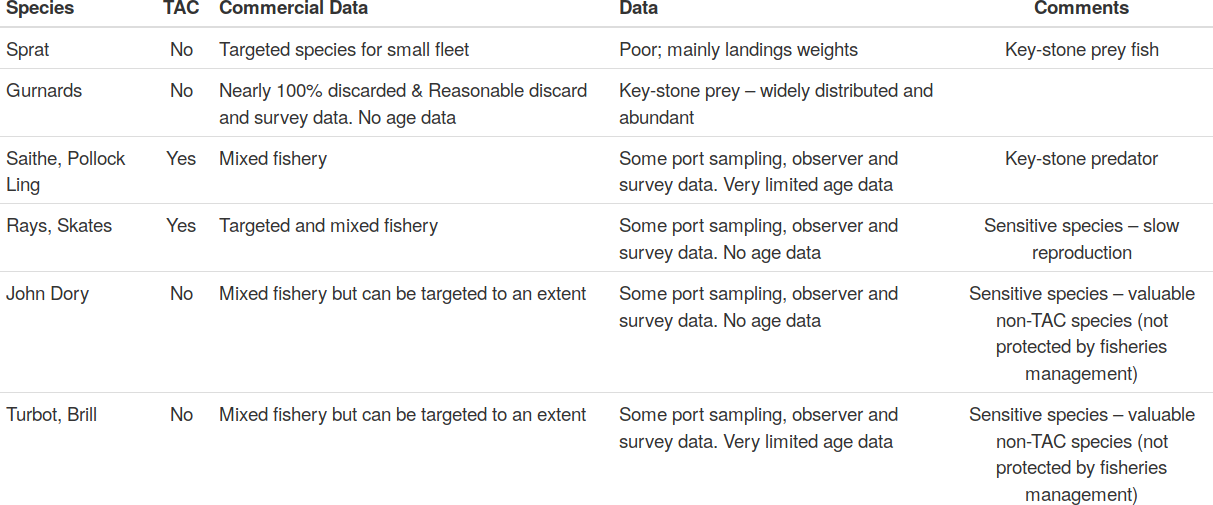
\includegraphics[width=6in]{/home/laurence/Desktop/sea++/mydas/final/report/tabs/stocks.png}\caption{Summary of potential study stocks.}\label{tab:stocks}
\end{table}
 
 
The final case studies were 
\href{https://3o2y9wugzp1kfxr5hvzgzq-on.drv.tw/MyDas/tasks/2/sprat.html}{sprat}, 
\href{https://3o2y9wugzp1kfxr5hvzgzq-on.drv.tw/MyDas/tasks/2/pollack.html}{pollack}, 
\href{https://3o2y9wugzp1kfxr5hvzgzq-on.drv.tw/MyDas/tasks/2/brill.html}{brill}, 
\href{https://3o2y9wugzp1kfxr5hvzgzq-on.drv.tw/MyDas/tasks/2/turbot.html}{turbot}, 
\href{https://3o2y9wugzp1kfxr5hvzgzq-on.drv.tw/MyDas/tasks/2/ray.html}{thornback ray}, 
\href{https://3o2y9wugzp1kfxr5hvzgzq-on.drv.tw/MyDas/tasks/2/lobster.html}{lobster} and 
\href{https://3o2y9wugzp1kfxr5hvzgzq-on.drv.tw/MyDas/tasks/2/razor.html}{razor clams} as these represent a range of life histories, and have a variety of roles in maintaining the structure of pelagic and demersal communities. The data on vertebrate life histories were accessed directly from \href{https://3o2y9wugzp1kfxr5hvzgzq-on.drv.tw/MyDas/tasks/1/stocks.html}{fishnets}. 

\begin{figure*}[h!]\centering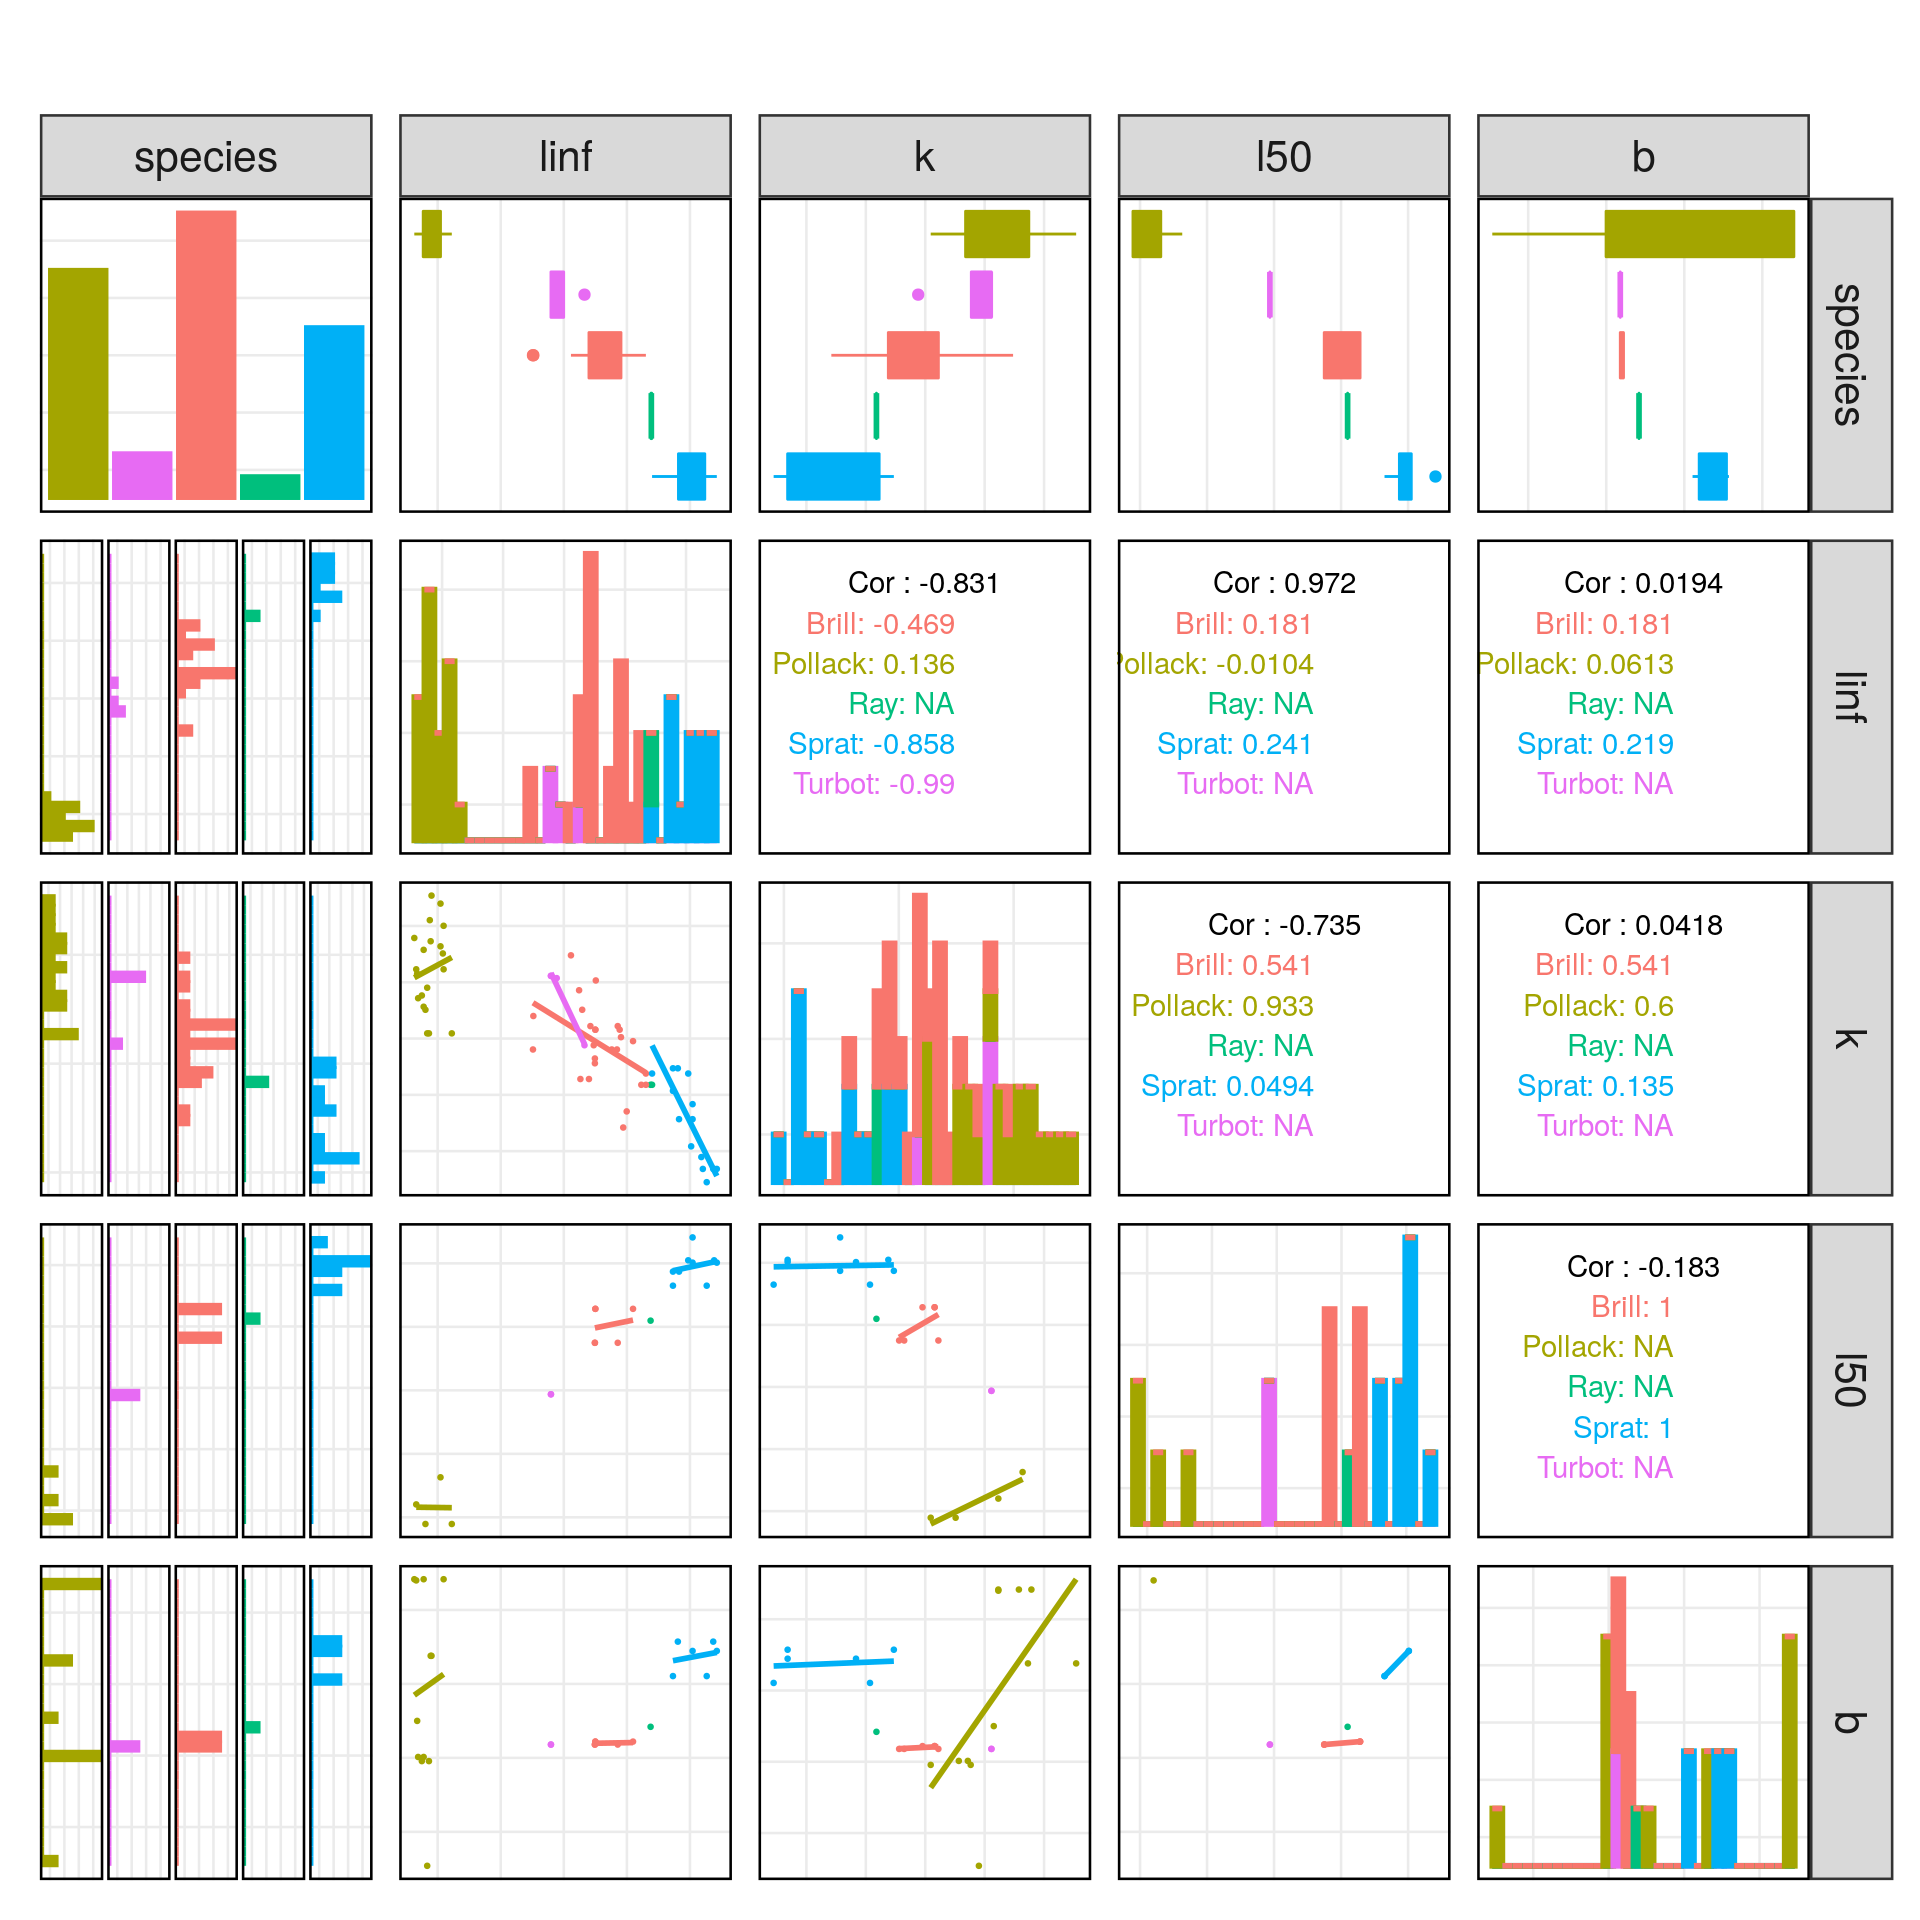
\includegraphics[width=6in]{figs/1-pairwise-1.png}\caption{Life history parameters for case study vertebrate stocks.}\label{fig:stocks}
\end{figure*}

 

\newpage\section{Data Collation}
The project relied on existing datasets rather than collecting new data and collating these data ran in parallel with other tasks. As well as Marine Institute data datasets were also obtained from ICES\footnote{\url{https://www.ices.dk/marine-data/dataset-collections/Pages/default.aspx}} and the JRC\footnote{\url{https://stecf.jrc.ec.europa.eu/dd/medbs/ram}}. While life history parameters were obtained from Fishbase\footnote{\url{http://www.fishbase.org/search.php}} and fishnets\footnote{\url{https://github.com/fishnets/fishnets}}, and stock assessment inputs and outputs from stockassessment.org\footnote{\url{https://www.stockassessment.org}}.

A database was designed see the \hyperref[appendix:db]{database summary} in the Appendix. These data were \href{https://3o2y9wugzp1kfxr5hvzgzq-on.drv.tw/MyDas/tasks/1/stockprioritisation.nb.html}{summarised} to help identify the case studies. To select the case studies a key dataset were the life history parameters. Many studies have shown that relationships between life history traits exists for processes such as growth, maturity and natural mortality. For data poor stocks, where information on key processes is lacking, life history theory can therefore be used allowing simulation models to be developed.  See the vignette on \href{https://3o2y9wugzp1kfxr5hvzgzq-on.drv.tw/MyDas/vignettes/conditioning.html}{conditioning Operating Models} on life history parameters. 

The various preliminary analyses based on the datasets compiled during MyDas in addition to life history theory are archived on \url{https://drive.google.com/open?id=1rR917GQhDm_b9bzCCxorwBAWvaTVDbix}{google drive}. %\coilin{[it says this folder is currently in the trash ;o) ]}.




\newpage\section{Assessment Methods}
%\textit{Method and simulation framework development and implementation](https://github.com/laurieKell/mydas/wiki/3-Method-and-simulation-framework-development-and-implementation). A number of data-limited methods exist. In order to compare the performance of these methods it would be useful to implement them all in the same framework, e.g. R. New methods may also be developed in the same framework.}

A number of data-limited methods already exist, in order to compare their performance they need to be run in a common framework. Therefore methods were interfaced to R, using the Fishery Library in R (\textbf{FLR}) \citep{kell2007flr} a toolset that is composed of a variety of packages, covering the various steps in the fisheries advice and simulation workflow. Using \textbf{FLR} means that advantage can be taken of existing methods, and that dissemination and support is easier and will be maintained after the life of the project. 

To identify the appropriate advice given the quality of data rules ICES classifies stock assessments into six \href{http://www.ices.dk/sites/pub/Publication Reports/Advice/2015/2015/General_context_of_ICES_advice_2015.pdf}{categories} on the basis of the available data, e.g. total landings, indices of abundance, length frequency and age data. 

\begin{description}[rightmargin=\dimexpr\linewidth-15cm-\leftmargin\relax]
 \item[Category 1: stocks with quantitative assessments]  Full analytical assessments and forecasts as well as stocks with quantitative assessments based on production models.

\item[Category  2: stocks  with  analytical  assessments  that  are  only  treated  qualitatively] 
Quantitative assessments and forecasts which for a variety of reasons are considered indicative of trends in fishing mortality, recruitment, and biomass.

\item[Category 3: stocks for which survey based assessments indicate trends] 
Survey or other indices are available that provide reliable indications of trends in stock metrics, such as total mortality, recruitment, and biomass.

\item[Category 4: stocks for which only reliable catch data are available] 
Time series of catch can be used to approximate MSY.

\item[Category 5: landings only]
Only landings data are available.

\item[Category 6: negligible landings]
Landings are negligible in comparison to discards and stocks that are  primarily caught as bycatch species in other targeted fisheries 
\end{description}


For data limited stocks a number of methods already exist, for example the ICES Working Group on Category 3 and 4 stocks \href{ 
http://www.ices.dk/sites/pub/Publication Reports/Expert Group Report/acom/2017/WKMSYCAT34/01 WKMSYCAT34 REPORT 2017.pdf}{(WGMSYCAT34)} has been working on rules for survey-based assessments which indicate trends in stock status (Category 3) or for which only catch data are available (Category 4). 

Data limited methods in use worldwide were summarised in a \href{https://docs.google.com/spreadsheets/d/17_qQdzDY41ZrL0yT6QtHpUR4_ydxx_xfCh4GiDqYymU/edit?usp=sharing}{google spreadsheet}. Following which five catch and three length based methods, were then selected for simulationn testing. The choice of methods was based on the availablity of code, whether the method had been peer reviewed and the appropriateness of estimated quantities for use as proxy reference points. The methods were then simulation tested \citep{pons2019catchlen} in order to select the best catch and length-only methods.


\subsubsection*{Catch Only}

Catch-only assessment methods evaluated were Catch-Maximum Sustainable Yield \citep[Catch-MSY][]{martell2013simple}, Depletion Based  Stock Reduction Analysis \citep[DBSRA][]{dick2011depletion}, Simple Stock Synthesis \citep[SSS][]{cope2013implementing}, an extension of Catch-MSY (CMSY), and State Space Catch Only Method \citep[SSCOM][]{thorson2015catch}. Length based methods evaluated were Length Based Spawning Potential Ratio \citep[LBSPR][]{hordyk2014novel,hordyk2015evaluation}, Length-Based Integrated Mixed Effects \citep[LIME][]{rudd2017accounting}, and Length-Based Bayesian \citep[LBB][]{froese2018new}.

Catch-MSY  is based on stock reduction analysis (SRA) that assume a Schaefer biomass dynamic model. Inputs are a time series of removals, priors for the population rate of increase at low population size ($r$), carrying capacity ($K$), and a probability distribution of stock depletion in the final year. CMSY, extends Catch-MSY by using a Monte-Carlo filter to fix systematic biases in the Catch-MSY. 

DBSRA further modifies the SRA approach by using Monte Carlo draws from the parameter distributions for M, $F_{MSY}/M$, $B_{MSY}/B_0$, depletion, and age at maturity ($A_{mat}$) to separate total biomass into immature and mature biomass using a delay-difference production model. 

SSS is based on Stock Synthesis  \citep{methot2013stock}, and fixes all parameters in a Stock Synthesis model except for initial recruitment ($lnR_0$). An artificial index of abundance that represents the relative stock biomass is used for fitting where the first value of the index is 1, and the value in the final year represents depletion (i.e. the proportion of the population left in the final year). Values of steepness ($h$) and depletion are randomly drawn from a specified distribution using a Monte Carlo approach and $lnR_0$ is then estimated. 

SSCOM is a Bayesian state-space model that integrates across three stochastic functional forms, variation in effort, population dynamics and fishing efficiency. 

\subsubsection*{Length Only}


LBSPR, estimates the proportion of the unfished reproductive potential per recruit  (SPR) under a given level of fishing pressure. In an exploited population is calculated as a function of the ratio of fishing mortality to natural mortality ($F/M$), selectivity, and the two life-history ratios $M/k$ and $L_m/L_{\infty}$; where k is the von Bertalanffy growth coefficient, $L_m$ is the size of maturity and $L_{\infty}$ is asymptotic size. The inputs are length at maturity specified in terms of $L_{50}$ and $L_{95}$ (the size at which 50\% and 95\% of a population matures) and length frequency data. LBSPR is an equilibrium based method and assumes asymptotic selectivity, von Bertalanffy growth, length at-age is normally distributed, rates of natural mortality are constant across adult age classes, recruitment is constant over time, and growth rates remain constant across the cohorts within a stock. 

LIME like LBSPR uses biological information and the length composition of the catch to estimate F and SPR. Unlike LBSPR, however, it does not assume equilibrium conditions and uses mixed effects to  estimate changes in recruitment and fishing mortality separately over time. 

LBB is a simple and fast method for estimating relative stock size that uses a Bayesian Monte Carlo Markov Chain (MCMC) approach. LBB uses pre-specified priors on parameters, and thus, technically does not require any inputs other than to length frequency data. It does provides the user the option to specify priors for $L_{\infty}$, length at first capture ($L_c$), and relative natural mortality ($M/k$). $F/M$ is estimated over the age range represented in the length-frequency sample. 


\subsubsection*{Evaluation}

The methods were simulation tested for three life history types (short, medium and long-lived), three historical exploitation scenarios, and three depleted levels \citep{pons2019catchlen}. The results of the simulations are shown in Figure \ref{fig:cln}. Of the five catch based methods SSCOM performs poorly in terms of precison and bias, while SSS is the least bias DBSRA the most precise. The length based methods tend to perform less well than the catch based methods, while LIME is the least biased while LBSPR is the most precise.

\begin{figure*}[h!]\centering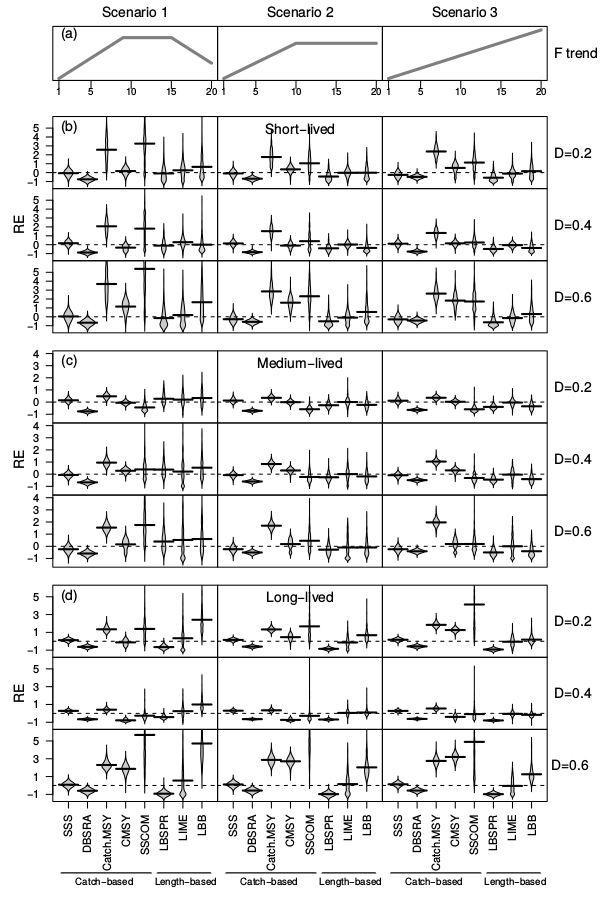
\includegraphics[width=6in]{figs/Figure_1.png}\label{fig:cln}\caption{Relative error (RE) in exploitation rate for all the catch-based and length-based models considered under the different harvest scenarios (a) and depletion scenarios for differing life histories, (b) short-lived, (c) medium-lived, and (d) long-lived.}
\end{figure*}

Bias and precision are both important factors to consider when assessing fish stocks. Bias reflects how close an estimate is to a known value; precision reflects reproducibility of the estimate. For example, if an assessment is to be re-conducted every year to monitor the impact of a management measure, a precise but biased method would be able to detect a trend better than an unbiased but imprecise method. Like a scientific instruments, this trade-off require calibration to correct for the bias, and such calibration can be explored using closed-loop simulations (i.e. MSE), where the choice of parameters and reference points in a Management Procedure are tuned (i.e. calibrated) to meet the desired management objectives as represented by the Operating Model. Thus, a biased method (e.g., DBSRA) may be preferable to one that is less biased, but more imprecise (e.g., LIME). Alternatively, imprecision can be addressed through the choice of the percentile (e.g., median being the 50\% percentile value) for the derived model output used by management (e.g., catch or SPR); assuming that the true value is contained within the parameter distribution. For example, instead of taking the median value, one could instead use the derived model output associated with the 40th percentile to incorporate risk tolerance as reflected in the calculated imprecision. Such an approach \citep{Ralston2011meta} is used in fisheries management systems to directly incorporate scientific uncertainty (both bias and imprecision), and can also be explored and tuned using MSE.

The best performing catch-only methods were SSS and DBSRA, SSS was the least biased method while DBSRA was the most precise. A problem with SSS is that it is based on SS3 and so is a complicated method that requires a lot of assumptions in the form of fixed parameters. DBSRA in contrast is based on a biomass based stock production function and so requires fewer assumptions, it also allows data poor and data rich assessments to be compared, i.e. if an index of abundance could be developed then an ICES Category 3 assessment could be converted into a Category 1 assessment. This allows the value of information to be evaluated. Therefore DBSRA was selected for further evaluation.  

Both LBSPR and LIME use the same inputs, the main difference is that LIME is a non-equilibrium method, takes longer to run than LBSPR and ofen failed to converge, so although LIME estimates are less biased than LBSPR it is likely to perform poorly in closed loop simulations. LBB performed poorly in terms of both bias and precision. Therefore LBSPR was selected for the next stage of simulation evaluation.



\newpage\section{Framework}
The majority of fish stocks worldwide lack sufficient data on which to base quantitative assessments. In some cases Management Strategy Evaluation \citep[MSE][]{10.1093/icesjms/fst232} has been used to develop harvest control rules (HCRs) based on empirical indicators that follow trends in survey estimates of abundance, catch rates or size composition. %Such rules have the advantage of being more easily understood by asset and stakeholders, also using  complex model-based assessments does not necessarily ensure a more robust management. %An alternative is to use model-based strategies which are attractive because they may be linked to the stock assessment results and generally have a greater capacity to “learn” about stock productivity. 

A reason for the use of MSE is because it is recognised that the robustness of advice depends on the combination of data, estimation method, choice of reference points as well as the rules used to set management action, i.e. the Management Procedure (MP). When conducting MSE an Operating Model (OM) is used to represent the dynamics of system being managed, and control actions from an MP are fed back into the OM so that its influence on the stock and hence on future fisheries data is propagated through the stock and fishery dynamics. 

Conducting MSE requires six steps; namely i) identification of management objectives; ii) selection of hypotheses for the OM; iii) conditioning the OM based on data and knowledge, and possible weighting and rejection of hypotheses; iv) identifying candidate management strategies; v) running the Management Procedure (MP) as a feedback control in order to simulate the long-term impact of management; and then vi) identifying the MPs that robustly meet management objectives. 

The MSE framework was based on the Fishery Library in R \citep[\href{http://www.flr-project.org/}{FLR}][]{kell2007flr}, which comprises a variety of packages that cover the various steps in the fisheries advice and simulation workflow. Using \textbf{FLR} means that advantage can be taken of existing methods, and that dissemination and support is easier and will be maintained after the life of the project. Under MyDas development focused on two main packages \textbf{FLife} and \textbf{mydas}. \textbf{FLife} is a package for modelling life history relationships and \textbf{mydas} provides a set of tools for simulation and conducting Management Strategy Evaluation (MSE) by providing wrappers for the various assessment methods, implementing Observation Error Models (OEMs) to simulate empirical indicators and other datasets, and to model harvest control rules (HCRs).

\textbf{FLife} was used to  condition OMs based on life history relationships and ecological theory, MP were then implemented using \textbf{mydas}. The link between the OM and the MP is the \href{https://3o2y9wugzp1kfxr5hvzgzq-on.drv.tw/MyDas/vignettes/oem.html}{OEM}, which generates fishery-dependent or independent resource monitoring data. The OEM models the uncertainties due to sampling and limited data and so mimics the types of data currently required for each assessment method. In addition the types of a data that could be made available in the future,

Simulation tests were also performed without feedback where the OEM was used to generate datasets from the OM. This allows the performance of the candidate methods to be compared, since if there is little correlation between the estimates of reference points and status from a candidate method and the OM then there is little point in running that method in the MSE. Tests were performed for a 
\href{https://3o2y9wugzp1kfxr5hvzgzq-on.drv.tw/MyDas/tasks/4/R/simtest-bd.pdf}{category 1 assessment} (a biomass dynamic assessment with catch and an index of abundance that estimates stock status and reference points), a \href{https://3o2y9wugzp1kfxr5hvzgzq-on.drv.tw/MyDas/tasks/4/R/simtest-lbspr.pdf}{category 3 assessment} that used a length based indicator, and a \href{https://3o2y9wugzp1kfxr5hvzgzq-on.drv.tw/MyDas/tasks/4/R/simtest-bdsra.pdf}{category 4 assessment} for which only catch data are available.

\subsubsection*{Performance measures} 

Management objectives under the Descriptor 3 of the \href{http://ec.europa.eu/environment/marine/good-environmental-status/descriptor-3/index_en.htm}{Marine Stewardship Framework Directive} and the Common Fisheries Policy of the European Union mandate that stocks should be exploited sustainably consistent with high long-term yields, have full reproductive capacity in order to maintain stock biomass and that the proportion of older and larger individuals should be maintained (or increased) as they are indicators of a healthy stock. These general objectives can be mapped to performance measures, so that alternative management strategies can be compared from both in and outside the ICES framework. %%For example

A range of summary statistics are required to illustrate trade-offs between multiple potentially conflicting objectives. Although there are many potential summary statistics so that decision makers can choose between tangible options on the basis of actual projections rather than abstract concepts. Performance statistics should, however, ideally be few, informative and based on principle metrics such as `stock status’, `safety', `stability' and `yield'. It is also necessary to distinguish between technical summary statistics (i.e. those required to evaluate model fits and performance) and those required to evaluate management objectives. Examples of summary statistics include 


\begin{description}[labelindent=\parindent,noitemsep,topsep=0pt,parsep=0pt,partopsep=0pt]
 \item[Safety] Probability of avoiding a limit such as  $B_{lim}$ where recruitment is impaired
 \item[Status] Probability of achieving targets related to MSY, e.g.  $B_{MSY}$ and $F_{MSY}$
 \item[Yield] Annual or cumulative yields
 \item[Variability] Inter-annual variation in catches or stock status
\end{description}


%The assessment methods chosen for testing, reflect a range of data and knowledge requirements, these were [LBSPR](https://cran.r-project.org/web/packages/LBSPR/index.html) for length compostion data, [MLZ](https://github.com/cran/MLZ) for mean size, [mpb](http://www.flr-project.org/) a biomass dynamic model for catch and survey data and catch only.

%\subsubsection*{Knowledge requirements}

%Stock assessment methods commonly require choices to be made for difficult to estimate parameters, there a set of [priors and fixed](https://3o2y9wugzp1kfxr5hvzgzq-on.drv.tw/MyDas/tasks/4/R/priors.pdf) parameters for the methods in the google spreadsheet were generated. These include values for

%\begin{itemize}[labelindent=\parindent,noitemsep,topsep=0pt,parsep=0pt,partopsep=0pt]
% \item Growth: $L_{\infty}$, $k$, $t_{0}$	
% \item Length-weight relationship: $a$, $b$
% \item Maturity: $L_{MAX}$, $A_{MAX}$ 
% \item Selectivity: $s_{50}$, $s_{95}$,	
% \item Production function K, $B_{0}$, r,	
% \item Natural Mortality: $M$, $M/K$
% \item Reference Points: $F_{msy}$ $M$, $B_{msy}/K$
% \item Length based reference points: $L_{c}$, $L_{opt}$
% \item Stock recruitment relationship: Steepness $h$, $a$ of Beverton and Holt
% \item Recruitment variation 
% \item Depletion	
% \item Fecundity at age/length,
%\end{itemize}


   

\newpage\section{Simulations}
ICES is in the process of developing methods to identify MSY proxy reference points for data-limited stocks at the ICES Workshop On The Development Of Quantitative Assessment Methodologies Based On Life-History Traits, Exploitation Characteristics, And Other Relevant Parameters For Data-Limited Stocks \href{http://ices.dk/sites/pub/Publication Reports/Expert Group Report/Fisheries Resources Steering Group/2019/WKLIFEIX/WKLIFE_IX_2019.pdf}{(WKLIFE)}. \textbf{MyDas} contributed to this process by proposing and testing new assessment models and methods of establishing reference points and attended both WKLIFE VIII and IX. There are key differences with the ICES approach, however, since \textbf{MyDas} stocks are not currently assessed by ICES and \textbf{MyDas} focused on the available data for each stock first and then on methods, while the ICES approach focuses on the methods first and then applies a limited number of methods to a large number of stocks. 

The importance of the work of \textbf{MyDas} was recognised at WKLIFEVIII where recommendations for \href{http://ices.dk/sites/pub/Publication Reports/Expert Group Report/acom/2018/WKLIFEVIII/WKLIFEVIII_2018.pdf#page=42}{future directions} were made. Following this several examples based on the work of \textbf{MyDas} were made at WKLIFEIX. These included i) the use of life history theory to condition the OM used to evaluate the ICES advice rule proposed for \href{http://ices.dk/sites/pub/Publication Reports/Expert Group Report/Fisheries Resources Steering Group/2019/WKLIFEIX/WKLIFE_IX_2019.pdf#page=30}{category 3 and 4 stocks}; ii) Receiver Operating Characteristic (ROC) curves to explore the setting of appropriate 
\href{http://ices.dk/sites/pub/Publication Reports/Expert Group Report/Fisheries Resources Steering Group/2019/WKLIFEIX/WKLIFE_IX_2019.pdf#page=58}{reference levels} in the the catch rule; and iii) the use of trends in an index \href{http://ices.dk/sites/pub/Publication Reports/Expert Group Report/Fisheries Resources Steering Group/2019/WKLIFEIX/WKLIFE_IX_2019.pdf#page=64}{without a reference level}. It was also recommended to use the methods of \textbf{MyDas} to evaluate the robustness of SPiCT based upon the development of Operating Models developed under \href{http://ices.dk/sites/pub/Publication Reports/Expert Group Report/Fisheries Resources Steering Group/2019/WKLIFEIX/WKLIFE_IX_2019.pdf#page=138}{MyDas}.

For stocks with analytical assessments (i.e. category 1 and 2 stocks), the advice rules applied by ICES are consistent with the objective of achieving MSY. For stocks in categories 3 and 4 ICES uses MSY proxy reference points as part of a Precautionary Approach to provide advice on the status of the stock and exploitation. The $F_{MSY}$ proxy corresponds to the exploitation rate that will provide maximum long-term yield, while the $MSY_{Btrigger}$ proxy corresponds to the stock size that triggers a cautious response; i.e. advises a reduced fishing mortality relative to $F_{MSY}$ proxy in order to allow the stock to rebuild. 

%%\\
\textit{Advice Rule}

For stocks with $MSY$ proxy reference points not derived from an assessment model, ICES uses a generic rule of the form 
 
\begin{equation}C_{y+1}=C_{current}rfb\end{equation}

where $C_{current}$ is the catch either in the most recent year available (typically $y-1$) or the average over a number of recent years (e.g. $y-n, ... ,y-1$), $r$ should account for the trend in stock biomass ($r>0$; with $r=1$ if there is no trend), $f$  is a proxy for the ratio $F_{MSY}/$(current exploitation) and $b=$ min(1,proxy for the ratio (current stock size)/($MSY_{Btrigger}$)). The later is in effect a hockey stick type HCR. 

$f$ is derived from length based indicators and a number of potential length based reference point and indicators\footnote{\url{http://ices.dk/sites/pub/Publication Reports/Guidelines and Policies/16.04.03.02_Category_3-4_Reference_Points.pdf}} have been identified by ICES for stocks in categories 3 and 4 (see Table \ref{tab:lib}) 

\begin{table}[h!]\centering
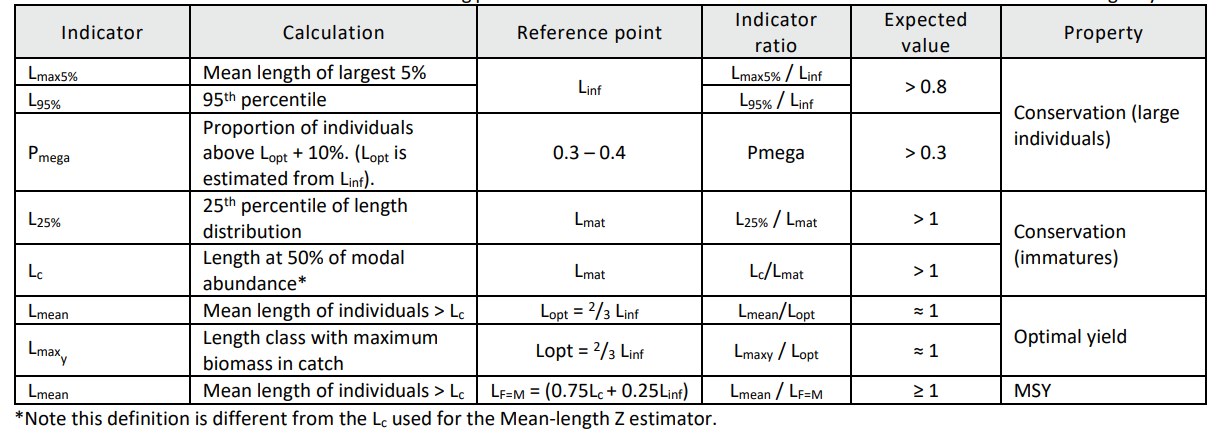
\includegraphics[width=\textwidth]{figs/lib.png}
\caption{Length based indicators.} 
\label{tab:lib}
\end{table}

The \textbf{mydas} package includes methods to simulate length frequency data and estimate indicators; Figure \ref{fig:ompollack} shows an OM based on pollack that was used to simulate indicators (Figure \ref{fig:libsim}).

\begin{figure}[h!]\centering
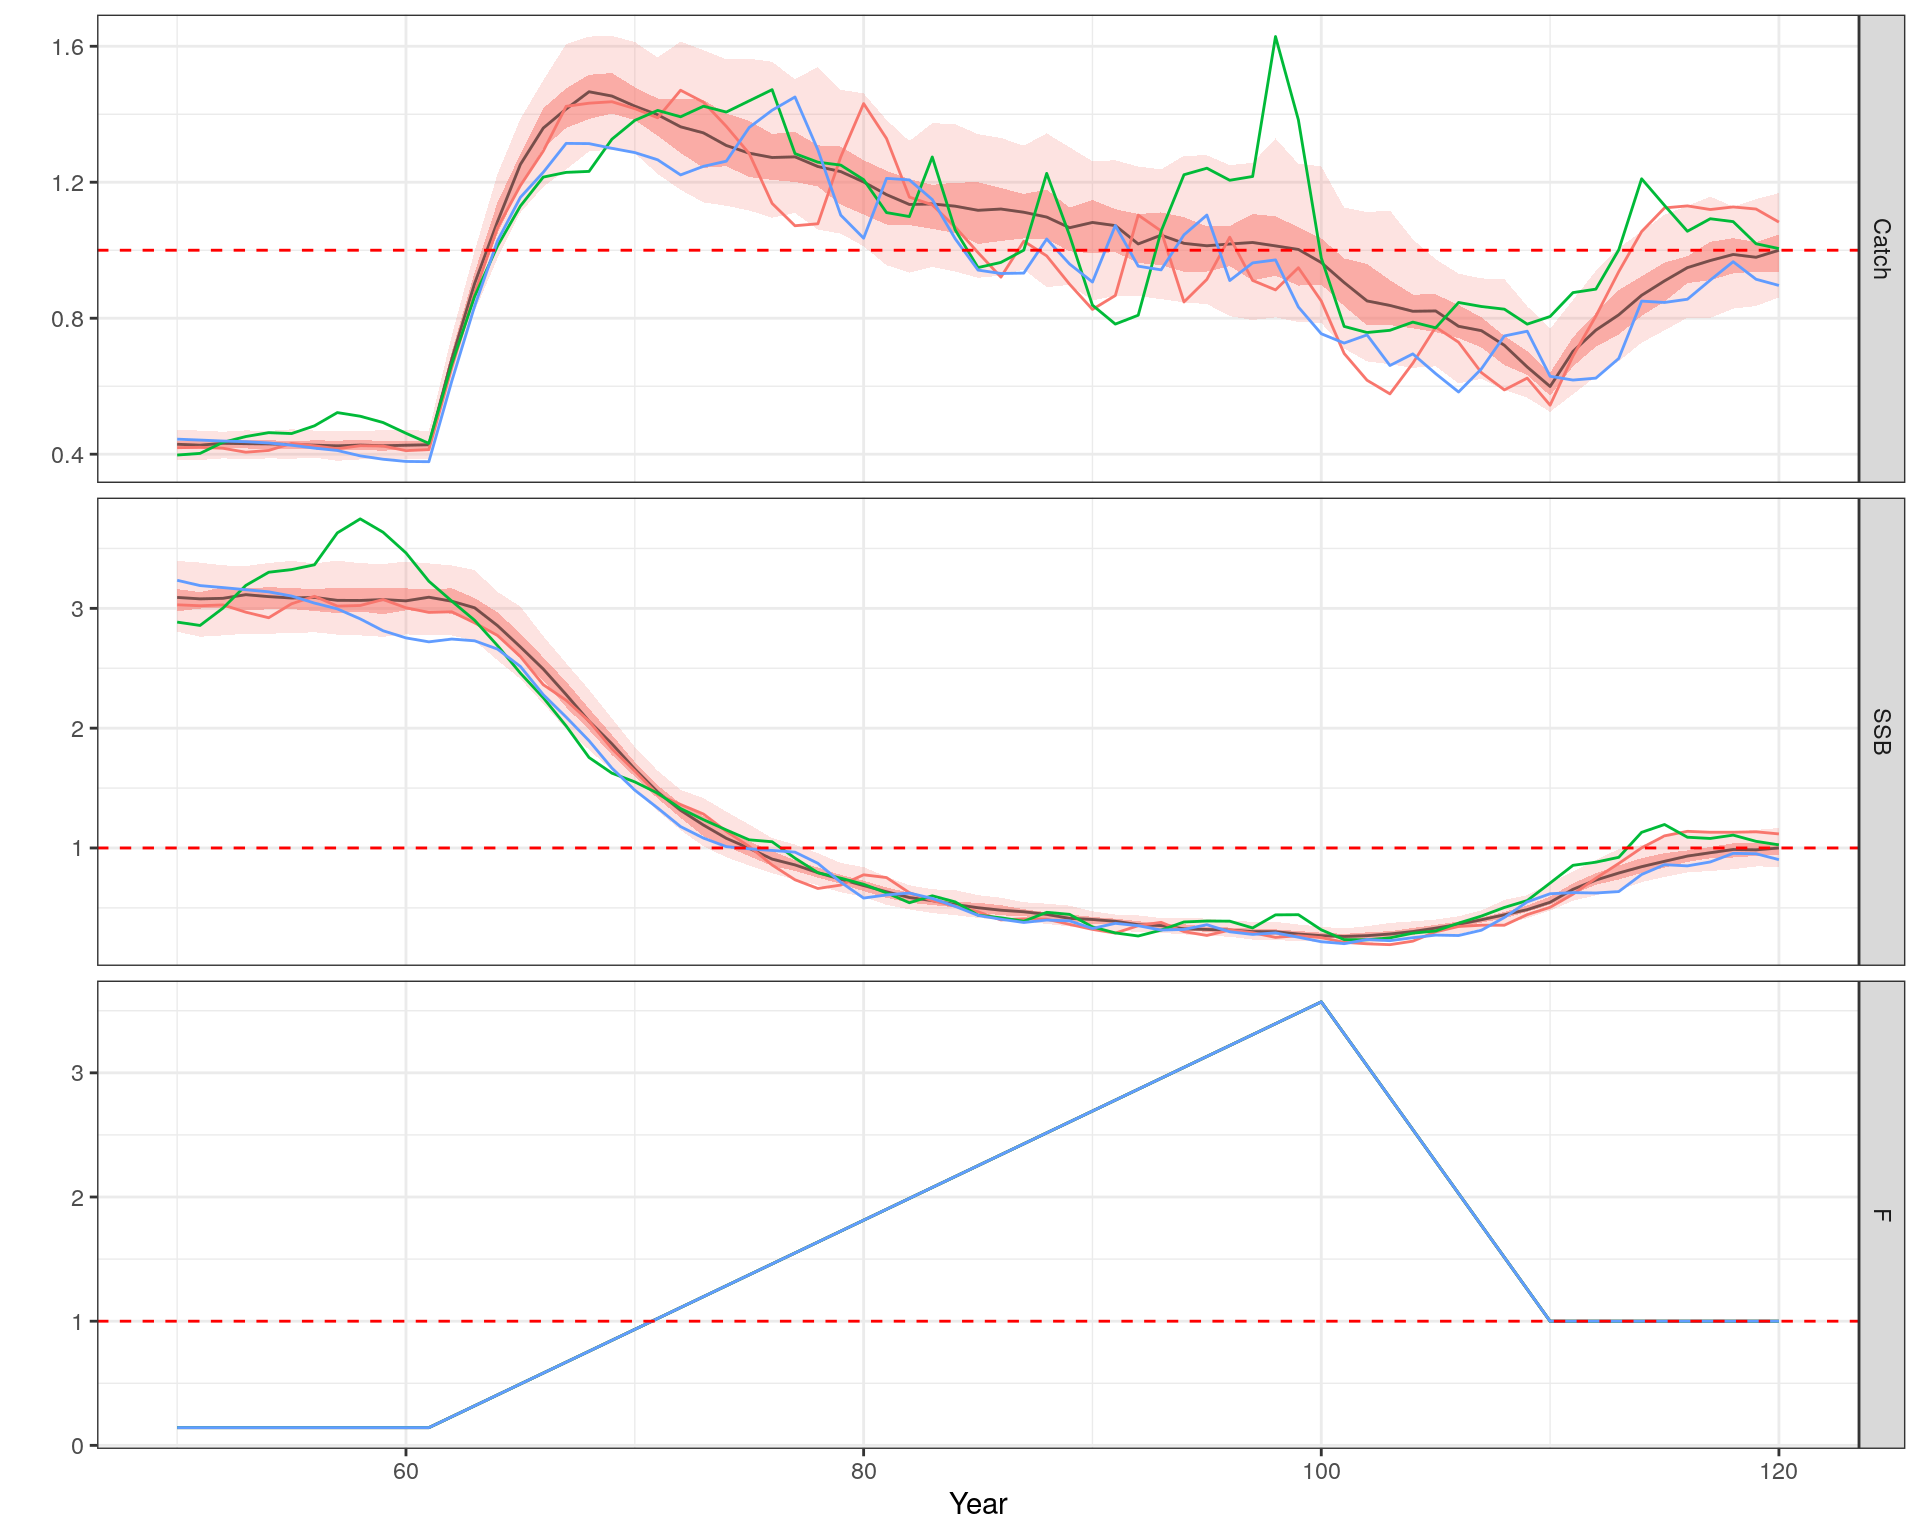
\includegraphics[width=\textwidth]{figs/roc-finalts-pollack-1.png}
\caption{Time series of simulated length based indicators, compared to $F/F_{MSY}$}
\label{fig:ompollack}
\end{figure}

\begin{figure}[h!]\centering
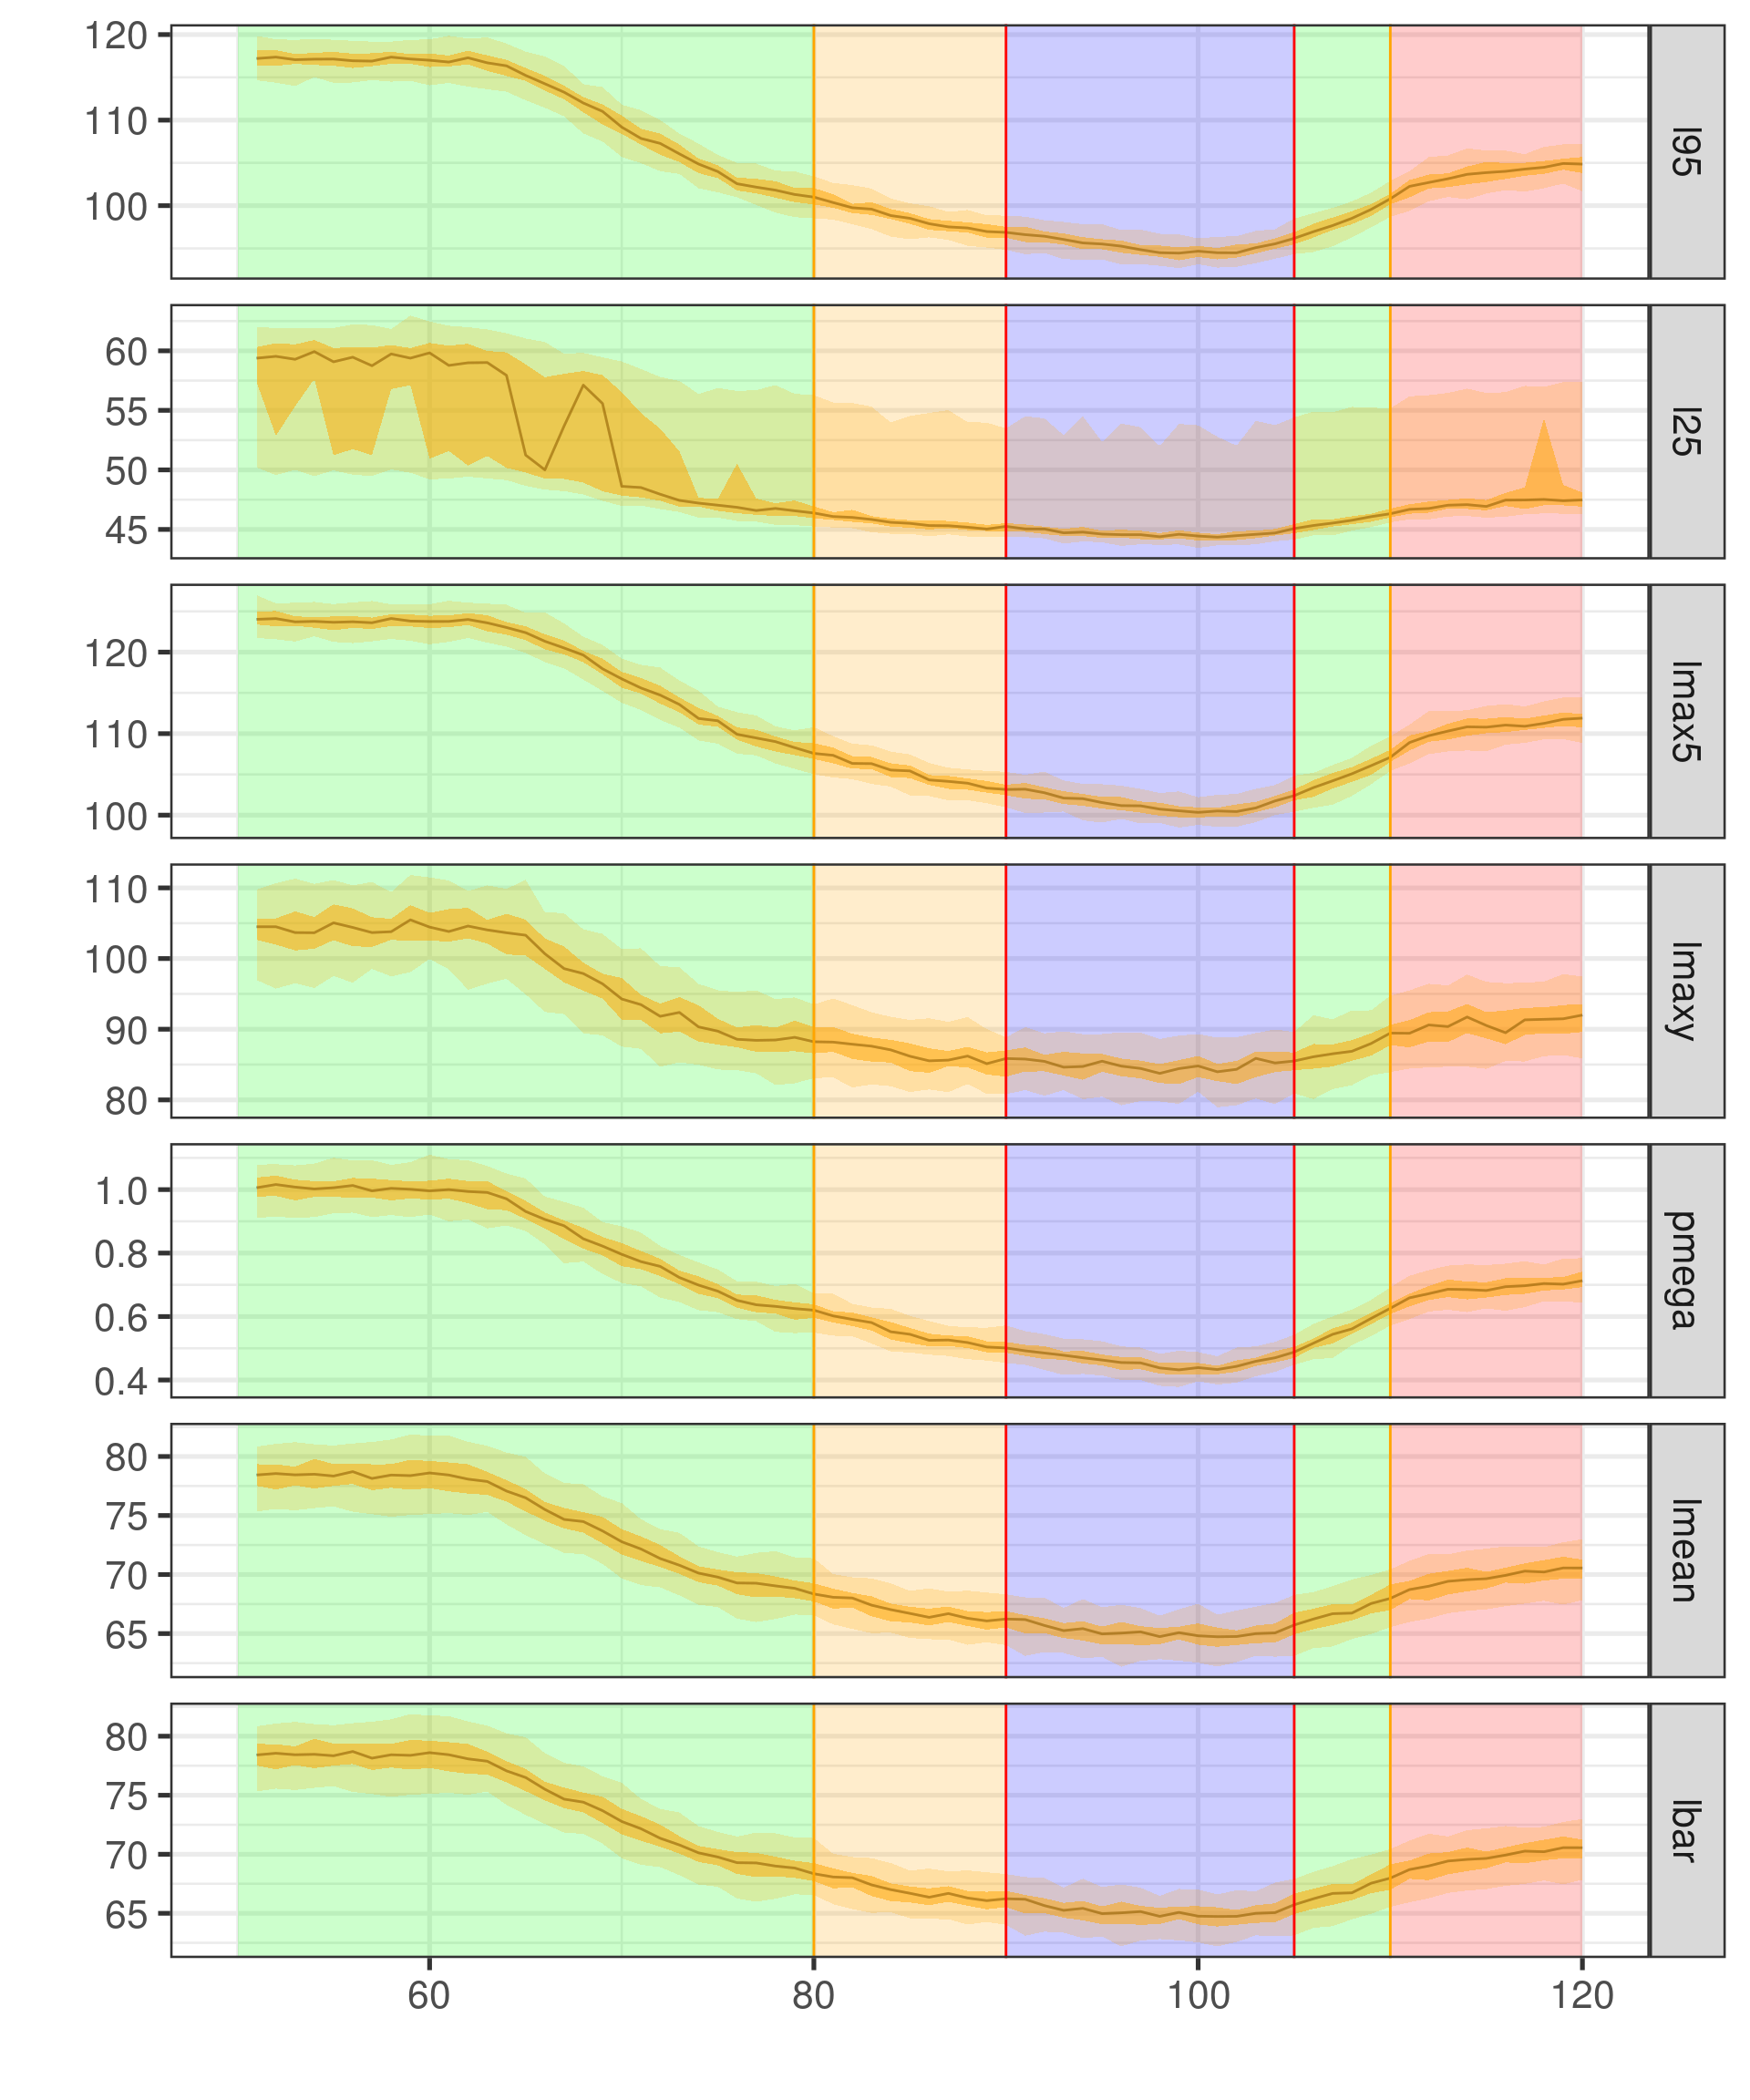
\includegraphics[width=\textwidth]{figs/roc-finalinds-1.png}
\caption{Time series of simulated length based indicators, compared to $F/F_{MSY}$}
\label{fig:libsim}
\end{figure}

To ensure that advice based on such indicators is precautionary, Management Strategy Evaluation was used to evaluate an empirical rule of the form $C_{y+1}=C_{current}rfb$ that bases catch advice on recent catches, information from a biomass survey index ($r$), length based indicators ($f$) and proxy MSY reference point ($b$) \citep{fischer2019hcr}. The OM was conditioned on life histories using the method developed by \textbf{MyDas} .The performance of the rule varied substantially between stocks, and the risk of breaching limit reference points was inversely correlated to the von Bertalanffy growth parameter $k$. Stocks with $k>0.32$  had a high probability of stock collapse. It was shown that a single generic catch rule cannot be applied across all life-histories, and management should instead be linked to life-history traits, and in particular, the nature of the time series. This supported the premise of \textbf{MyDas} that to develop robust management it is important to consider the nature of the stock dynamics, knowledge and data. 
Counter-intuitively the catch rule performed poorly for the more productive stocks (those with higher $k$) compared to the less productive stocks (with lower $k$). The performance of the catch rule, however, is an emergent property of the interaction between the operating model and the catch rule. Therefore this is an important result, which would not have been apparent without the work of our manuscript.

The advised catch was mainly influenced by one component of the rule (the trend in the relative index of abundance) and biomass trends for stocks with higher $k$) are inherently more variable, which in turn leads to higher fluctuations in catch. Therefore when managed by the ICES catch rule, the stocks with higher $k$) were more likely to collapse during simulation. This behaviour can be attributed to an initial rapid recovery, which resulted in an increase in catch. Once the stocks started to decline again, however, catch was not reduced quickly enough to avoid stock collapse. This undesirable feature is caused by the design of the catch rule, which bases the newly advised catch on the previous catch and observed data with a time-lag. Since the less productive stocks (those with low $k$) were also less variable, the catch rule was sufficiently reactive to avoid stock collapse.

Therefore two papers are currently being drafted. The first used Receiver Operating Characteristic (ROC) curves used to explore the setting of appropriate reference levels in the $f$ component of the catch rule for the \textbf{MyDas} case studies. In particular to explore how these depend on life-history traits and the nature of the time-series. The second evaluated the use of trends in an index without a reference level for pollack. To do this, a Management Strategy Evaluation (MSE) was conducted to evaluate an empirical harvest control rule (HCR) based on a trend in an index of
abundance. The Operating Model (OM) was conditioning on pollack life-history characteristics and the HCR was based on that used by the Commission for the Conservation of Southern Bluefin Tuna (CCSBT). The HCR has several parameters that require tuning \citep{hillary2015scientific}, i.e. the parameters are found by choosing values that best meet the objectives of asset and stakeholders; i.e. optimises the outcomes modelled as a reward function.\\
Preliminary work within {\bf{MyDas}} on the spectral decomposition of recruitment time series (\hyperref[appendix:spectral]{appendix}) provides a promising avenue to increase the realism of the simulated recruitment time series over simply increasing the process variability. 

\subsubsection*{Derivation of a continuous HCR}
Work is also ongoing looking at equilibria for \href{https://drive.google.com/open?id=1ldTJfrVxNsIHD9s9W0jyNaeedLZqDIPS}{coupled biomass systems} this is potentially useful as it provides a theoretical basis for the development of Harvest Control Rules, and will allow the properties of candidate HCRs to be explored analytically prior to setting up MSE simulations.




\newpage\section{Liason and Linkage}

%\textit{Liaison with Marine Institute](https://github.com/laurieKell/mydas/wiki/6-Liaison-with-Marine-Institute) The service provider is expected to meet on a regular basis with MI staff involved in the project: Monthly update meetings at the Marine Institute premises in Oranmore Galway with researcher providing the research services, 6-monthly progress reports and meetings at the Marine Institute with the researcher providing the research services and contract manager.

The service provider meet on a regular basis with Marine Institute staff involved in the project. While to ensure good communication between the consortium and the Marine Institute to ensure the project keeps focused and delivers. Therefore we will arrange monthly face-to-face meetings, make all code, data and results available on the cloud and in a suitable repository (e.g. github) and provide a web based interface for model results.\\


%Wider project 6-monthly progress reports and meetings at the Marine Institute will ensure the over-arching goals of the project are achieved.


Attendance at \href{http://ices.dk/sites/pub/Publication Reports/Expert Group Report/Fisheries Resources Steering Group/2019/WKLIFEIX/WKLIFE_IX_2019.pdf#page=30}{wklifeix: 4 Length-based approaches} and 
ICES WKLIFE \& Working Group for the Celtic Seas Ecoregion \href{https://www.ices.dk/community/groups/Pages/WGCSE.aspx}{(WGCSE)}


\textit{Linkage with other projects](https://github.com/laurieKell/mydas/wiki/7-Linkage-with-other-projects)
The service provider is required to link research output to the following projects: }


The MyDas framework was developed though case studies in collaboration with a range of partners, as well as the MI and ICES, these included the tuna Regional Management Fisheries Organisations (tRFMOs), the University of Washington and the JRC. These case studies resulted in a number of peer review manuscripts. 

\begin{itemize}
 \item Monkfish\\
 This project will develop in close collaboration with the Cullen Fellowship of Mr Luke Batts, co-supervised by Dr Hans Gerritsen (MI) and Dr C\'oil\'in Minto (GMIT). Active collaboration will occur with Tasks 3--5, as these are similarly proposed in the Cullen Fellowship where they are applied specifically to \textit{Lophius budegassa} and \textit{Lophius piscatorius} stocks in ICES areas VII-VIII.
 \item Pollock \\
 Active collaboration exists between GMIT and the Newport Research Cluster (e.g., \emph{Unlocking the Archive} project). Further collaboration and linkages will be built around data-poor assessment of pollock (liasing with the dedicated Scientific and Technical Officer working on pollock at the Furnace research facility). Both visits to Newport and group attendance at the monthly meetings will facilitate collaboration and crossover.
 \item DRuMFISH project \\
 The project will also link with the DGMARE project: ``Study on approaches to management for data-poor stocks in mixed fisheries (DRuMFISH)'' to which GMIT is a partner in the consortium. Methodological development from DRuMFISH (e.g., hierarchical methods) will be directly relevant to the present proposal. 
 \item CPV codes 71354500-9 Marine survey services 73112000-0 Marine research services 90712300-4 Marine conservation strategy planning 98360000-4 Marine services 77700000-7 Services incidental to fishing 73000000-2 Research and development services and related consultancy services 73110000-6 Research services 73200000-4 Research and development consultancy services 73210000-7 Research consultancy services.
 \item There are also other projects worldwide that can be link to e.g. the global group on stock assessment methods and the tRFMO MSE WG. 
 \end{itemize}

\begin{itemize}[labelindent=\parindent,noitemsep,topsep=0pt,parsep=0pt,partopsep=0pt]
 \item \textbf{Achievements}
 \item \textbf{Promises \& Differences}
 \item \textbf{What \& Why}
\end{itemize}

\href{http://ices.dk/sites/pub/Publication Reports/Expert Group Report/Fisheries Resources Steering Group/2019/WKLIFEIX/WKLIFE_IX_2019.pdf#page=30}{wklifeix: 4 Length-based approaches}

[wklifeix: ROC](http://ices.dk/sites/pub/Publication Reports/Expert Group Report/Fisheries Resources Steering Group/2019/WKLIFEIX/WKLIFE_IX_2019.pdf#page=58)

[wklifeix: hake](http://ices.dk/sites/pub/Publication Reports/Expert Group Report/Fisheries Resources Steering Group/2019/WKLIFEIX/WKLIFE_IX_2019.pdf#page=100)

[wklifeix: hake](http://ices.dk/sites/pub/Publication Reports/Expert Group Report/Fisheries Resources Steering Group/2019/WKLIFEIX/WKLIFE_IX_2019.pdf#page=101)

Evaluate further improvements to the performance of the WKMSYCat34 catch rule 3.2.1.
Focus on improving the catch rule for stocks with von Bertalanffy growth parameter
k>0.32, investigate more extensively the definition of the catch rule components and their
impact on performance, and investigate the possibility of alternative catch rules.
• Explore the operating model set-up for data-limited simulations, including sensitivity
analyses based on the Jacobian; e.g. elasticity analysis, on how the different life-history
and fishery parameters affect the simulated stock behaviour under exploitation, an analysis of the nature of time-series and trends of observable stock characteristics (such as
fishery-dependent and -independent metrics) and how the knowledge gained can be
used to further improve the performance of catch rules



 + **The International Council of the Exploration of the Sea (ICES)** is in the process of developing methods to identify MSY proxy reference points for data-limited stocks ([WKLIFE](http://ices.dk/sites/pub/Publication Reports/Expert Group Report/Fisheries Resources Steering Group/2019/WKLIFEIX/WKLIFE_IX_2019.pdf)). The service provider is required to contribute to this process by proposing and testing new assessment models and methods of establishing reference points and will be expected to attend up to 4 one-week meetings at ICES headquarters in Copenhagen. However there are key differences with the ICES approach. Since this research contract will include stocks not currently assessed by ICES; focusing on the available data for each stock first and on the methods second; the ICES approach focuses on the methods first and then applies a limited number of methods to a large number of stocks.


\newpage\clearpage
\bibliography{mydas.bib}
\bibliographystyle{abbrvnat}

\flushbottom
\newpage

%% APPENDICES
\newpage

\begin{appendices}

\newpage\section{}

\subsection{Database}\label{appendix:db}

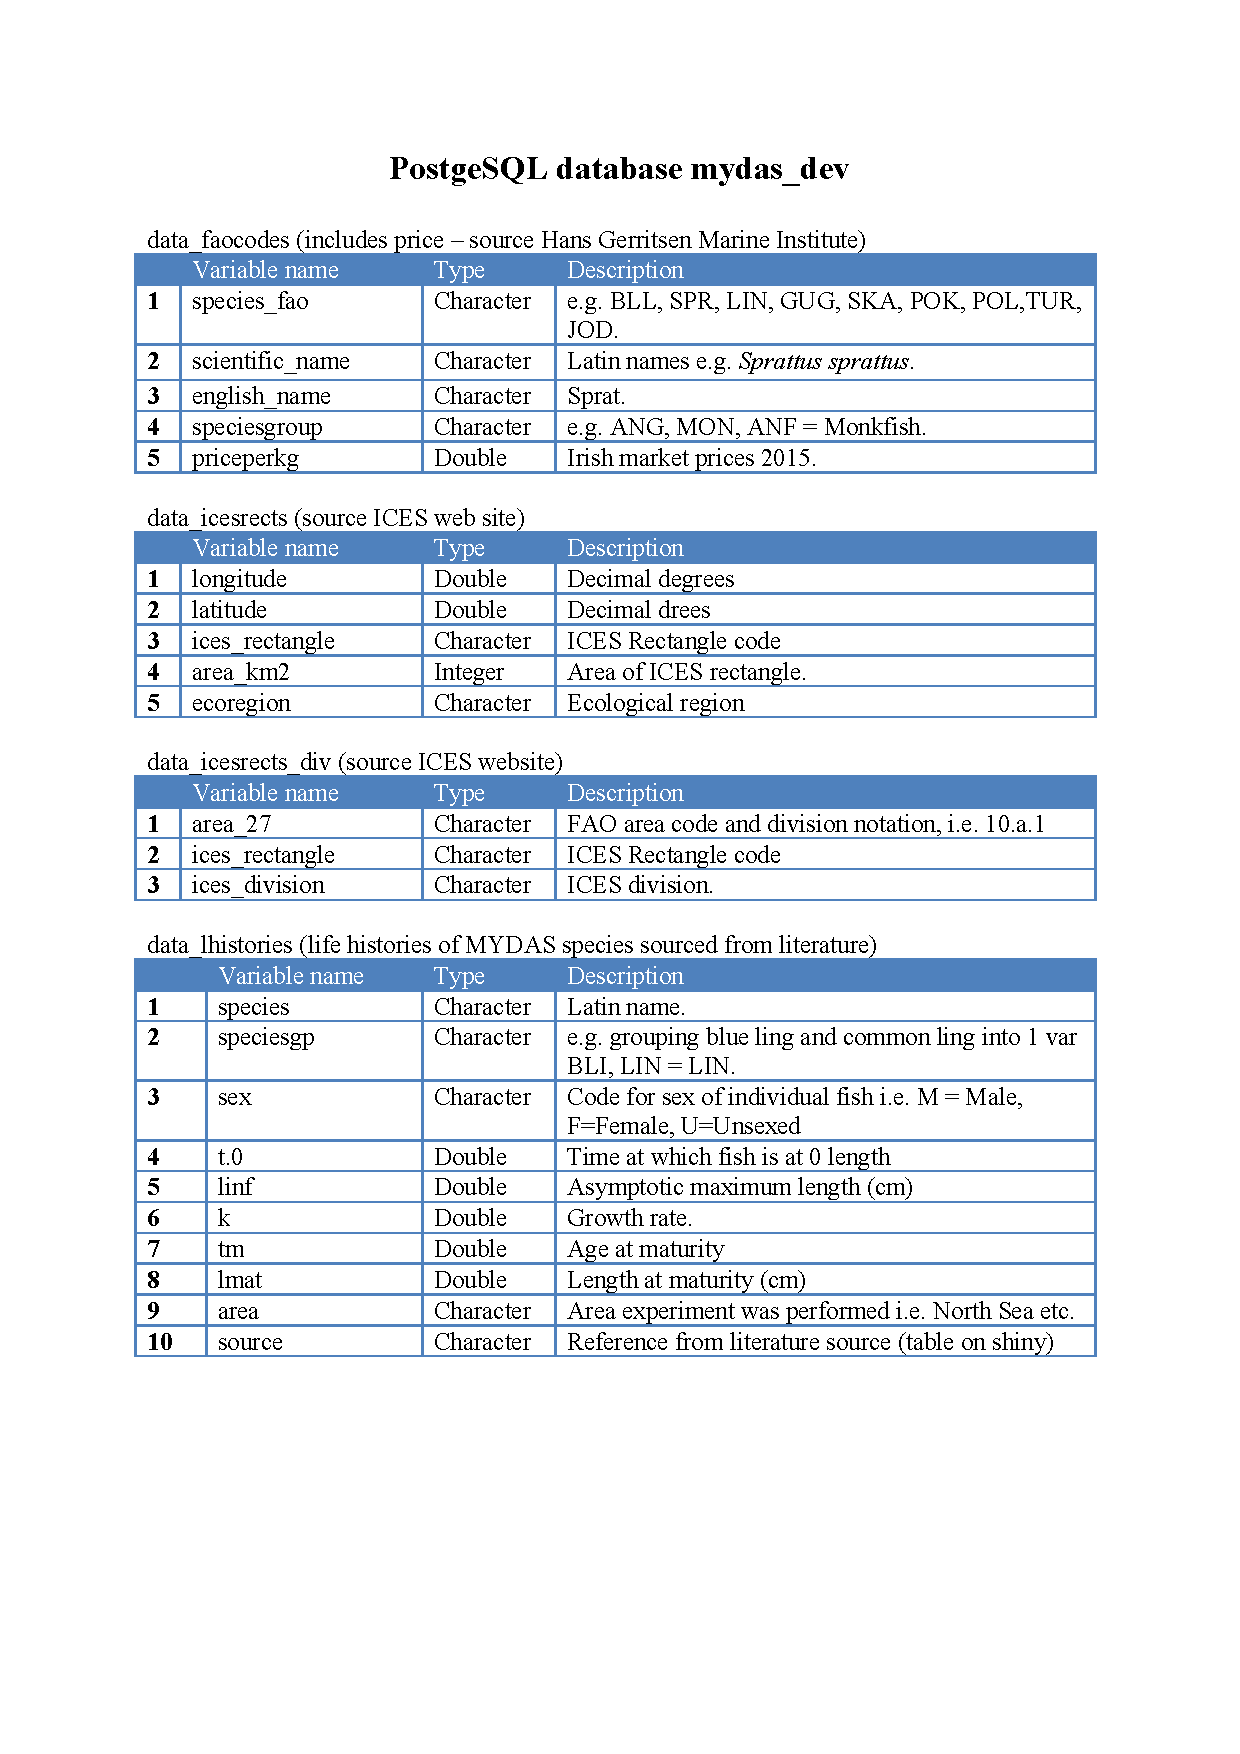
\includepdf[pages=1-5,pagecommand={},width=\textwidth]{include/Databasedescripton.pdf}

\subsection{Dataset Summary}\label{appendix:datsets}

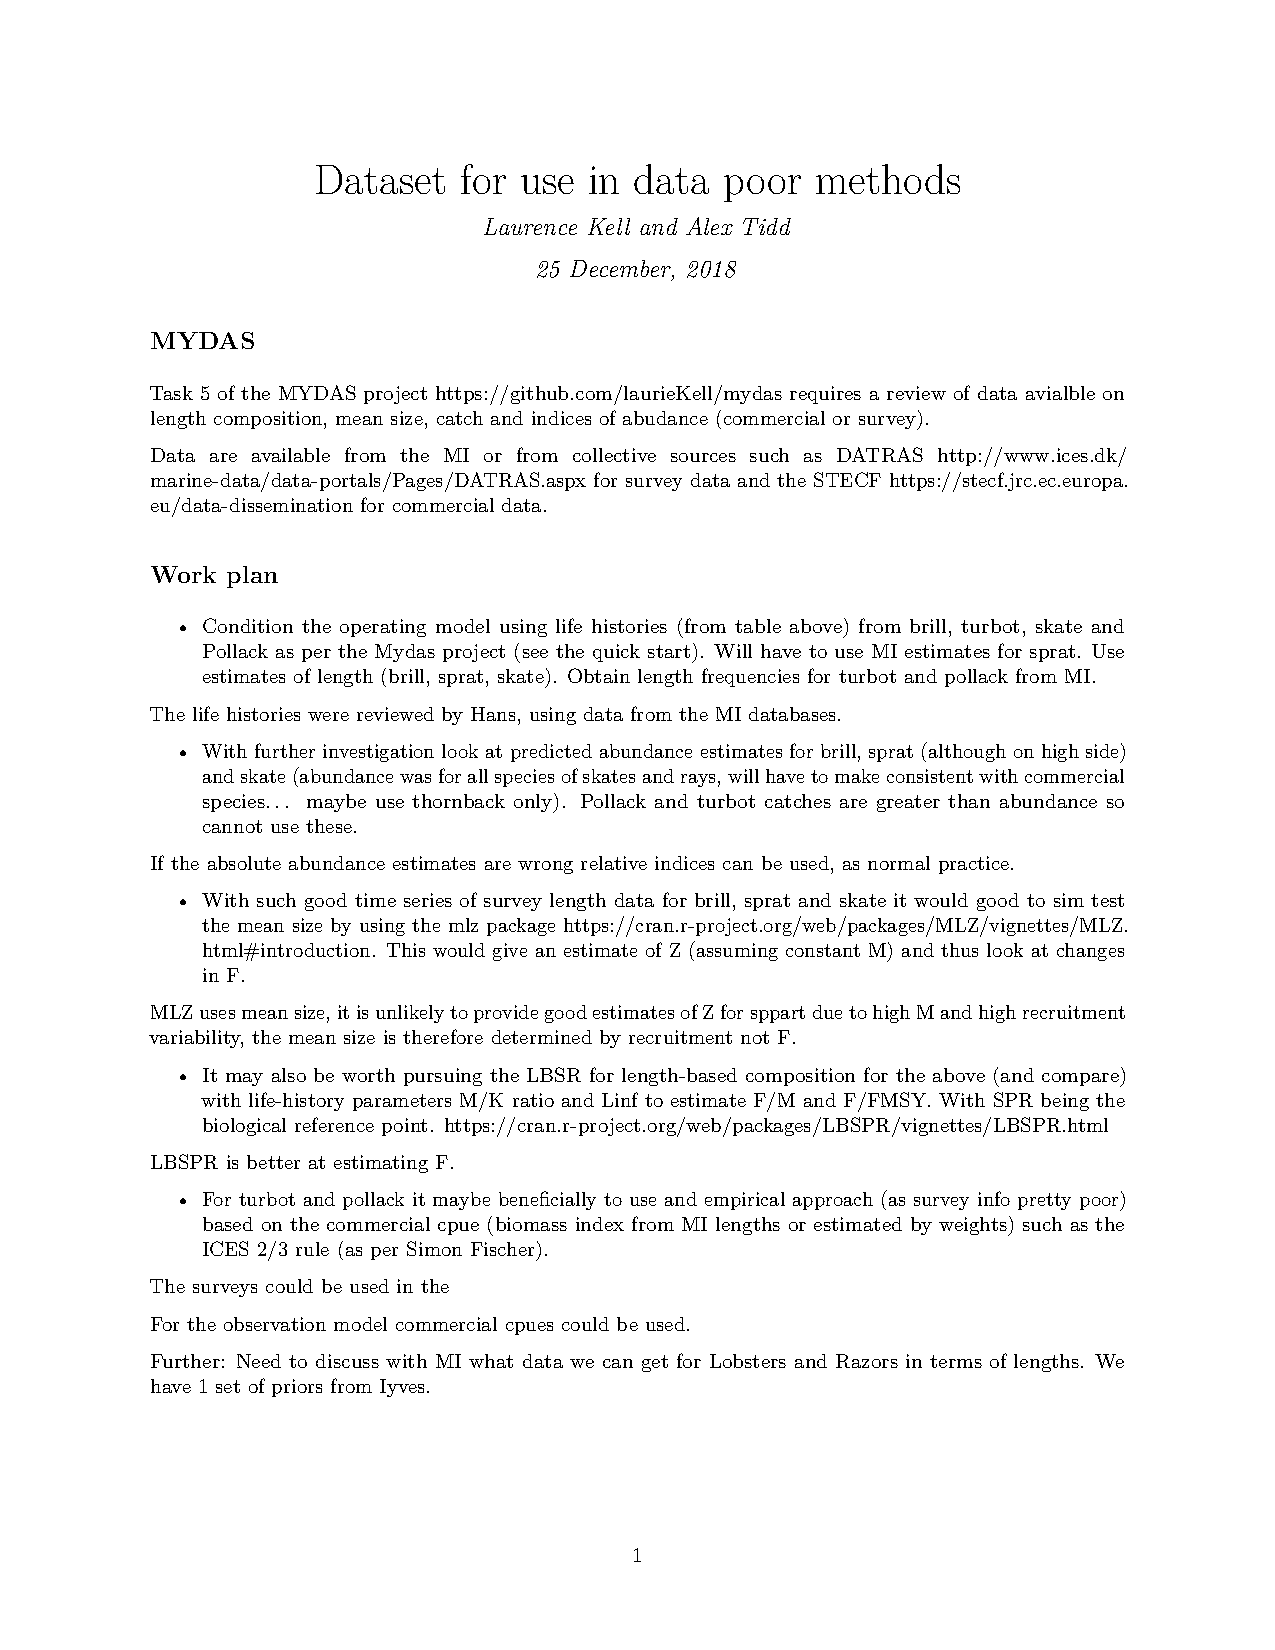
\includepdf[pages=-,pagecommand={},width=\textwidth]{include/dataSmry.pdf}

\section{Peer Review Papers}

\subsection{Linking the performance of a data-limited empirical catch rule to life-history traits}
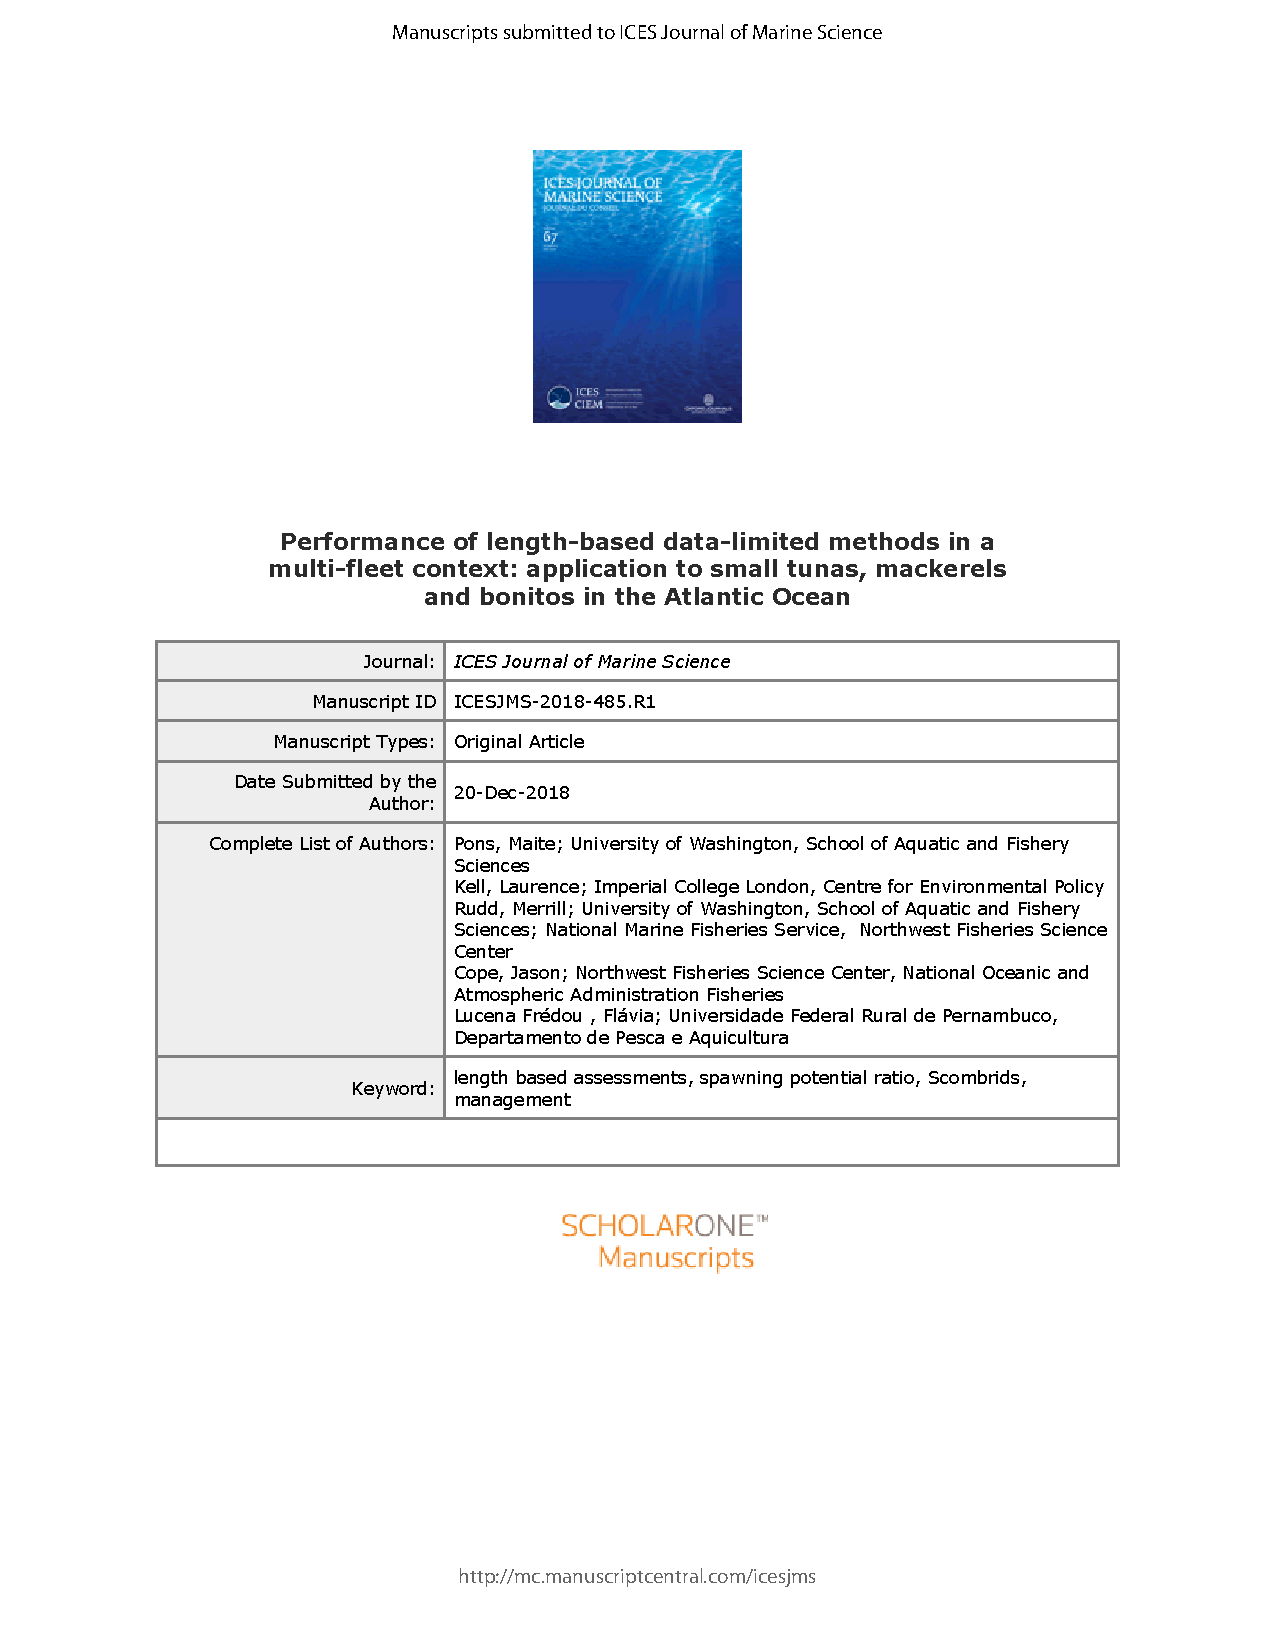
\includepdf[pages=-,pagecommand={},width=\textwidth]{include/ICESJMS_2019_350_R1_Proof_hi.pdf}

\subsection{Performance of length-based data-limited methods in a multi-fleet context}
\includepdf[pages=-,pagecommand={},width=\textwidth]{include/12553688_File000007_240052393.pdf}

\subsubsection{ROC}
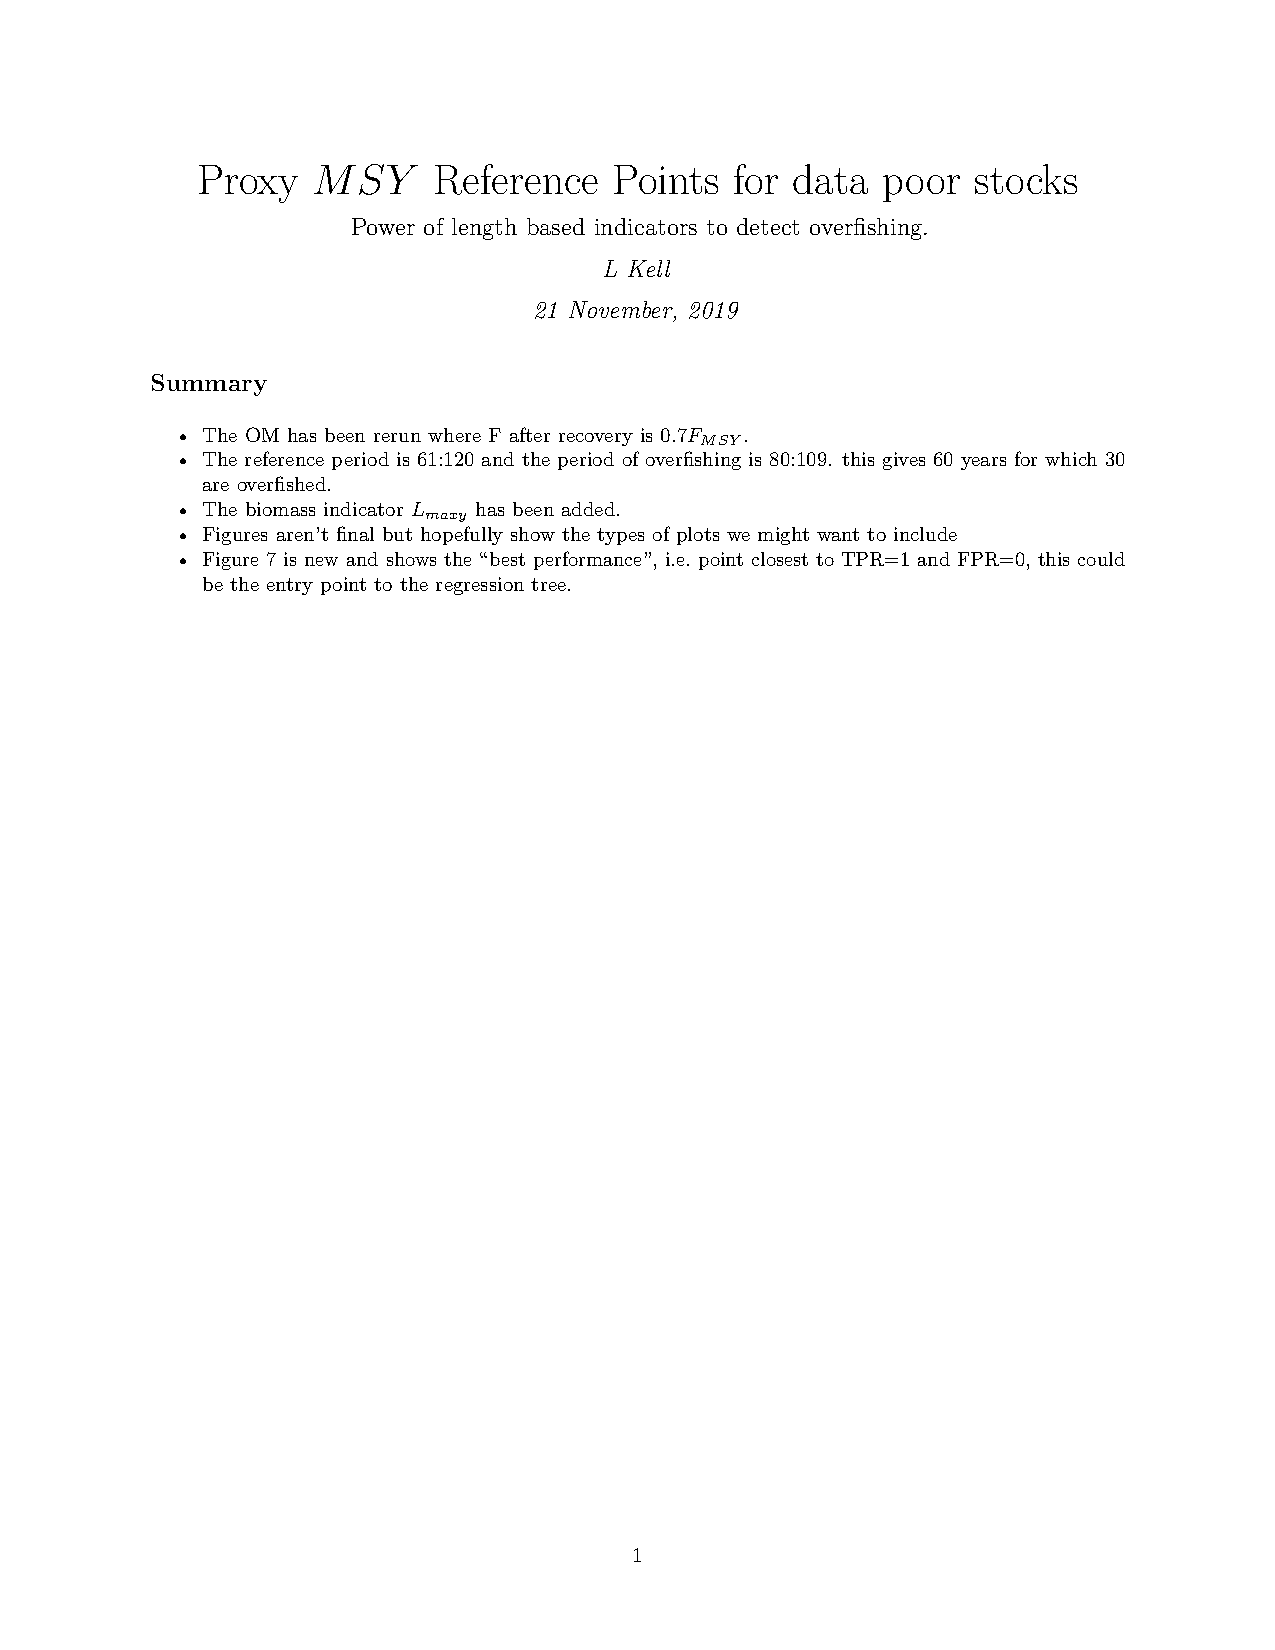
\includepdf[pages=1,pagecommand={},width=\textwidth]{include/roc.pdf}

\subsubsection{Pareto}
\includepdf[pages=1,pagecommand={},width=\textwidth]{include/pareto.pdf}

\end{appendices}

\end{document}


%\href[y9wugzp1kfxr5hvzgzq-on.drv.tw/MyDas/presentations.html}{presentations)
%\href[y9wugzp1kfxr5hvzgzq-on.drv.tw/MyDas/tasks/1/stockprioritisation.nb.html}{prioritisation)
%\href[y9wugzp1kfxr5hvzgzq-on.drv.tw/MyDas/tasks/1/stocks.html}{stocks)
%\href[y9wugzp1kfxr5hvzgzq-on.drv.tw/MyDas/tasks/2/brill.html}{brill)
%\href[y9wugzp1kfxr5hvzgzq-on.drv.tw/MyDas/tasks/2/lobster.html}{lobster)
%\href[y9wugzp1kfxr5hvzgzq-on.drv.tw/MyDas/tasks/2/pollack.html}{pollack)
%\href[y9wugzp1kfxr5hvzgzq-on.drv.tw/MyDas/tasks/2/ray.html}{ray)
%\href[y9wugzp1kfxr5hvzgzq-on.drv.tw/MyDas/tasks/2/razor.html}{razor)
%\href[y9wugzp1kfxr5hvzgzq-on.drv.tw/MyDas/tasks/2/sprat.html}{sprat)
%\href[y9wugzp1kfxr5hvzgzq-on.drv.tw/MyDas/tasks/2/turbot.html}{turbot))
%\href[y9wugzp1kfxr5hvzgzq-on.drv.tw/MyDas/tasks.html}{tasks)
 

ln /home/laurence-kell/Desktop/projects/mydas/tasks/2/Databasedescripton.pdf /home/laurence-kell/Desktop/projects/mydas/report/include/Databasedescripton.pdf
ln /home/laurence-kell/Desktop/projects/mydas/tasks/2/dataSmry.pdf           /home/laurence-kell/Desktop/projects/mydas/report/include/dataSmry.pdf
ln /home/laurence-kell/Desktop/projects/mydas/papers/length/ICESJMS-2018-485.R1_Proof_hi.pdf /home/laurence-kell/Desktop/projects/mydas/report/include/ICESJMS_2019_350_R1_Proof_hi.pdf
ln /home/laurence-kell/Desktop/projects/mydas/papers/catchLen/12553688_File000007_240052393.pdf /home/laurence-kell/Desktop/projects/mydas/report/include/12553688_File000007_240052393.pdf
ln /home/laurence-kell/Desktop/projects/mydas/papers/roc/roc.pdf /home/laurence-kell/Desktop/projects/mydas/report/include/roc.pdf
ln /home/laurence-kell/Desktop/projects/mydas/papers/pareto/pareto.pdf /home/laurence-kell/Desktop/projects/mydas/report/include/pareto.pdf
